\RequirePackage{fix-cm}
\documentclass[oneside, a4paper]{book}
\usepackage[a4paper,width=150mm,top=25mm,bottom=25mm,bindingoffset=6mm]{geometry}

% Required for inserting images
\usepackage{eso-pic,graphicx}
% misc
\usepackage{caption}
\DeclareCaptionType{equ}[][]
%\captionsetup[equ]{labelformat=empty}
\usepackage{subcaption}
\usepackage{multicol}
\usepackage{float}
\usepackage{adjustbox} % oversized table

% appendix
\usepackage[toc]{appendix}

% Default font to sans serif
\renewcommand{\familydefault}{\sfdefault}
\RequirePackage[T1]{fontenc} 
\RequirePackage[tt=false, type1=true]{libertine} 
\RequirePackage[varqu]{zi4} 
% \RequirePackage[libertine]{newtxmath}

% chapters and headers
\usepackage[Conny]{fncychap}

\usepackage{fancyhdr}
\pagestyle{fancy}
\renewcommand{\headrulewidth}{0.1pt}
\renewcommand{\chaptermark}[1]{\markboth{\MakeUppercase{\textsf{{#1}}}}{}}
\renewcommand{\sectionmark}[1]{\markright{\MakeUppercase{\textsf{\thesection\ #1}}}{} }

% section styling
\usepackage{titlesec}

% algorithms
\usepackage{algorithm}
\usepackage{algpseudocode}

% theorems and definitions
\usepackage{amsthm}
\newtheorem{definition}{Definition}


% FAT FONTS
\usepackage{bm} % bold fonts in math mode
\newcommand\fat[1]{{\boldmath{\textbf{#1}}}}
\newcommand\emphasis[1]{{\scshape\bfseries#1}}

% mathematical fonts and graphics
\usepackage{mathtools}
\usepackage{xfrac} % sfrac for diagonal slashes in fractions
\usepackage{amsfonts} % math fonts
\usepackage{amssymb} % more math symbols (supsetneq etc.)
\usepackage{dbnsymb}
\usepackage{dsfont} % math fonts
\usepackage{bbm} % mathbb fonts
\usepackage{mathrsfs} % fancy swirly font
\usepackage{gensymb} % degree sign

% draw graphs
\usepackage[inline]{asymptote}
\usepackage{qtree}
\usepackage{tikz}

% nicer fractions
\usepackage{xfrac}
% cancel terms
\usepackage{cancel}

% units
\usepackage{siunitx}

% plots
\usepackage{pgfplots}
\usepackage{pgfplotstable}
\usepgfplotslibrary{external}
\usepgfplotslibrary{patchplots}
\usepgfplotslibrary{groupplots}
\pgfplotsset{compat=1.18} 
\tikzexternalize[prefix=tikz,optimize=false]


% define the Spectral_r color scheme
\usepackage{xcolor}
\definecolor{Spectral0}{RGB}{158, 1, 66}
\definecolor{Spectral1}{RGB}{213, 62, 79}
\definecolor{Spectral2}{RGB}{244, 109, 67}
\definecolor{Spectral3}{RGB}{253, 174, 97}
\definecolor{Spectral4}{RGB}{254,224,139}
\definecolor{Spectral5}{RGB}{255,255,191}
\definecolor{Spectral6}{RGB}{230,245,152}
\definecolor{Spectral7}{RGB}{171,221,164}
\definecolor{Spectral8}{RGB}{102,204,204}
\definecolor{Spectral9}{RGB}{50,136,189}
\definecolor{Spectral10}{RGB}{94,79,162}
\pgfplotsset{
  colormap={Spectral_r}{
    rgb255(0cm)=(94,79,162)         % 0.0
    rgb255(1cm)=(50,136,189)        % 0.1
    rgb255(2cm)=(102,204,204)       % 0.2
    rgb255(3cm)=(171,221,164)       % 0.3
    rgb255(4cm)=(230,245,152)       % 0.4
    rgb255(5cm)=(255,255,191)       % 0.5
    rgb255(6cm)=(254,224,139)       % 0.6
    rgb255(7cm)=(253,174,97)        % 0.7
    rgb255(8cm)=(244,109,67)        % 0.8
    rgb255(9cm)=(213,62,79)         % 0.9
    rgb255(10cm)=(158,1,66)         % 1.0
    }
}


% get width of given text
\usepackage{calc}

% define a horizontal spacer
\newcommand\horizontalspacer[0]{\vspace{5pt}\noindent\textcolor{lightgray}{\rule{\textwidth}{1mm}}
\vspace{5pt}}

% clickable links
\usepackage{hyperref}
\hypersetup{
    colorlinks,
    citecolor=black,
    filecolor=black,
    linkcolor=black,
    urlcolor=black
}
\renewcommand{\itemautorefname}{Item}
% citations
\usepackage[
  backend=biber,
  sorting=none,
  style=ieee,
  doi=false,
  % isbn=false,
  url=false,
  eprint=false
]{biblatex}
\addbibresource{refs.bib}

% fancy boxes
\usepackage{fancybox}
\newcommand{\equationnamed}[2]{%
  \setlength{\fboxsep}{2pt} % padding inside box
  \setlength{\fboxrule}{0.01pt}
  \begin{center}
    \begin{minipage}{\textwidth}
      \begin{center}\textsc{#1}\end{center}
      #2
    \end{minipage}
  \end{center}
}
\newcommand{\equationnamedbox}[2]{%
  \setlength{\fboxsep}{5pt} % padding inside box
  \setlength{\fboxrule}{0.01pt}
  \begin{center}
    \fbox{
      \begin{minipage}{0.4\textwidth}
        \begin{center}\emphasis{#1}\end{center}
        #2
      \end{minipage}
    }
  \end{center}
}

% labels to enum items
\usepackage{enumitem}

% make empty lines skip
% \usepackage{parskip}

% ~~~~~~~~~ TYPESETTING AND OTHER MACROS ~~~~~~~~~~~~~~~~~~~~~

\newenvironment{absolutelynopagebreak}
  {\par\nobreak\vfil\penalty0\vfilneg
   \vtop\bgroup}
  {\par\xdef\tpd{\the\prevdepth}\egroup
   \prevdepth=\tpd}

% ~~~~~~~~~ AFANCY CHAPTER HEADINGS ~~~~~~~~~~~~~~~~~~~~~~~~~~~
\makeatletter
\def\thickhrulefill{\leavevmode \leaders \hrule height 1ex \hfill \kern \z@}
\def\@makechapterhead#1{%
  %\vspace*{50\p@}%
  \vspace*{10\p@}%
  {\parindent \z@ \centering \reset@font
        \thickhrulefill\quad
        \scshape \@chapapp{} \thechapter
        \quad \thickhrulefill
        \par\nobreak
        \vspace*{10\p@}%
        \interlinepenalty\@M
        \hrule
        \vspace*{10\p@}%
        \Huge {\textbf{#1}} \par\nobreak
        \par
        \vspace*{10\p@}%
        \hrule
    \vskip 40\p@
    % \vskip 100\p@
  }}
\def\@makeschapterhead#1{%
  %\vspace*{50\p@}%
  \vspace*{10\p@}%
  {\parindent \z@ \centering \reset@font
        \thickhrulefill
        \par\nobreak
        \vspace*{10\p@}%
        \interlinepenalty\@M
        \hrule
        \vspace*{10\p@}%
        \Huge \bfseries #1\par\nobreak
        \par
        \vspace*{10\p@}%
        \hrule
    \vskip 40\p@
    % \vskip 100\p@
  }}

  
\usepackage[pdftex,outline]{contour}

% ~~~~~~~~~ ALGORITHM MACROS ~~~~~~~~~~~~~~~~~~~~~~~~~~~~~~~~~
\newcommand{\var}[1]{\text{\texttt{#1}}}
\newcommand{\func}[1]{\text{\textsl{#1}}}

\makeatletter
\newcounter{phase}[algorithm]
\newlength{\phaserulewidth}
\newcommand{\setphaserulewidth}{\setlength{\phaserulewidth}}
\newcommand{\Phase}[1]{%
  \vspace{-1.25ex}
  % Top phase rule
  \Statex\leavevmode\llap{\rule{\dimexpr\labelwidth+\labelsep}{\phaserulewidth}}\rule{\linewidth}{\phaserulewidth}
  \Statex\strut\refstepcounter{phase}\textit{Step ~\thephase~--~#1}% Phase text
  % Bottom phase rule
  % \vspace{-1.25ex}\Statex\leavevmode\llap{\rule{\dimexpr\labelwidth+\labelsep}{\phaserulewidth}}\rule{\linewidth}{\phaserulewidth}
  }

\makeatother
\makeatother

\setphaserulewidth{.1pt}

% ~~~~~~~~~ MATH MACROS ~~~~~~~~~~~~~~~~~~~~~~~~~~~~~~~~~~~~~~

% abs value macro
% \DeclarePairedDelimiter\abs{\lvert}{\rvert}
\newcommand\abs[1]{\left|#1\right|}
\newcommand\norm[1]{\left\lVert#1\right\rVert}
\newcommand\angled[1]{\left\langle#1\right\rangle}

\newcommand\dist[1]{\left|\left|#1\right|\right|}
\newcommand\arr[1]{\left\langle#1\right\rangle}

% define the laplace operator 
\newcommand*\Laplace{\mathop{}\!\mathbin\nabla^2}
\newcommand\vek[1]{\vec{\bm{#1}}}
\newcommand\mat[1]{{\mathds{#1}}}
\newcommand\br[1]{\left(#1\right)}

\DeclareMathOperator{\sgn}{sgn}
\DeclareMathOperator{\erf}{erf}

\DeclareMathOperator*{\argmax}{\arg\!\max}
\DeclareMathOperator*{\argmin}{\arg\!\min}

\newcommand\divergence{{\nabla\cdot}}


% ~~~~~~~~~ START ~~~~~~~~~~~~~~~~~~~~~~~~~~~~~~~~~~~~~~~~~~~

\captionsetup[figure]{font=footnotesize,labelfont=footnotesize,justification=centering}
\begin{document}
\begin{titlepage}
  \pagestyle{empty}

  \begin{center}
    \Huge\textbf{Simulating Incompressible Fluids with Weakly Coupled Rigid Bodies}\\
    \vspace{0.5cm}
    \Large{Julian Karrer}\\
    \vfill
    \Large
    % \contour{black}{\textcolor{white}{Lab Course}}\\
    % \contour{black}{\textcolor{white}{Master of Science in Computer Science}}\\
    \begin{figure}[H]
        \centering
        \includegraphics[width=1\textwidth]{images/title2.png}
    \end{figure}
    \vfill
    % \vspace{5.2cm}
    % \vspace{0.5cm}
    \large
    Faculty of Engineering\\
    Department of Computer Science\\
    Supervised by Prof. Dr.-Ing. Matthias Teschner\\
    \vspace{0.5cm}
    \includegraphics*[width=5cm]{images/ufr-logo.png}
  \end{center}
\end{titlepage}
% \captionsetup[figure]{font=normalsize,labelfont=normalsize}

\tableofcontents
\newpage

\chapter{Introduction}
This report aims to outline a complete implementation of a robust, fully GPU-parallel particle based solver for incompressible fluid flow problems with weakly coupled rigid bodies that can two-way interact with the fluid. The solver is efficient enough to make simulations with high spatial resolution and corresponding particle counts well into the millions feasible on a single machine with consumer hardware. Diffuse spray, foam and air bubbles are generated in a physically motivated way to enhance visual realism for simulations of sufficiently large spatial scale for such effects to occur. \\

The governing equations to be solved, namely the incompressible Navier-Stokes equations in Lagrangian form are introduced and discretized using the Smoothed Particle Hydrodynamics scheme, or SPH for short, in \autoref{chp:sph}. 

This leads to a set of equations that can be worked into a fluid solver in \autoref{chp:fluid}. Most challengingly, this solver must uphold incompressibility, leading to a pressure solver that must solve the pressure Poisson equation, in this case using a relaxed Jacobi solver with different choices of source term that lead to different behaviour of the solver. 

Once the fluid solver is completed, including one-way coupling to boundaries as discussed in \autoref{chp:rigid}, the remainder of the chapter discusses a second, rigid body solver, that uses an SPH-based surface representation to interact with the former and enable two-way interactions of rigid bodies with fluids. Challenges include a robust sampling of surfaces, the accurate calculation of the required volume and moments of mass of triangular meshes and 


\chapter{Smoothed Particle Hydrodynamics}\label{chp:sph}
    \section{Navier-Stokes Equations}\label{sec:navier-stokes}
    In order to develop a numerical solver for fluid flow problems, the respective governing equations must first be discussed. In the case of linearly viscous, incompressible fluid flow, the framework of continuum mechanics yields a set of equations called the \emphasis{Navier-Stokes equations}. Since the focus on this report is on the implementation of the solver, these equations are only very concisely outlined in the following and the interested reader is referred to more extensive works such as by \cite[Anderson]{anderson} or a previous report authored by the present writer \autocite{labcourse} for a more thorough derivation.

    \subsubsection{Lagrangian Continuum Mechanics}
    Since the flow problems in question occur not a microscopic scale, such as concerning the interaction of individual molecules, but a macroscopic scale instead, continuum mechanics is a suitable framework for the formulation of the governing equations. It assumes that the fluid is a continuum that is under deformation, wherein field quantities such as density, velocity etc. are convected with continuum elements as they deform, and makes use of the \emphasis{Material derivative} to apply the rules of calculus to these quantities \autocite{anderson}:
      \begin{equation}
        \frac{D}{Dt} := \underbrace{\frac{\partial}{\partial t}}_{\textit{local derivative}} + \underbrace{\br{\vek{v}\cdot \nabla}}_{\textit{convective derivative}}
      \end{equation}
    The first term represents the local derivative, or instantaneous rate of change of the quantity with respect to the continuum element, while the second describes the rate of change of the quantity at a fixed position due to the deformation of the continuum and consequently the convection of the continuum element with the velocity field $\vek{v}$. The frame of reference for each continuum element that is convected along with the velocity field is precisely the one in which the second term becomes zero, yielding the Lagrangian or so-called non-conservation form of the equations instead of the Eulerian form of the problem in which a static frame of reference is chosen \autocite{anderson}. We choose the Lagrangian representation in the following since the continuum itself is later discretized into particles that are advected with the flow and only quantities at particle positions will be of interest. An Eulerian discretization of the space within which the continuum exists could be chosen instead, but may be less suitable in application to free-surface flows with complex and dynamic boundary geometry \autocite{tutorial2019}.

    \subsubsection{Governing Equations}
    The governing equations can be derived from laws of conservation applied to the continuum. The first such conservation law is the \emphasis{conservation of mass} $\frac{Dm}{Dt}=0$, which can be transformed using either the Reynolds Transport theorem or the divergence theorem \autocite{labcourse} into the continuity equation of the form:
    \equationnamedbox{Continuity Equation}{
      \begin{equation}\label{eq:continuity}
        \frac{D\rho}{Dt} +\rho\br{\divergence \vek{v}} = 0
      \end{equation}
    }
    for incompressible flows, which has to hold across the entire volume integral over the fluid domain \autocite{anderson}. Since the flow is incompressible, the density of any fluid element must remain constant across a wide range of pressures, as will be assumed is the case of water. This assumption leads to two equivalent constraints posed by the continuity equation \autocite{continuum-intro}: 
    \begin{enumerate}
      \item $\frac{D\rho}{Dt}=0$, the density of any fluid element cannot change \label{enum:continuity-equation-constraint-den}
      \item $\divergence\vek{v}=0$ the velocity field of the fluid must be divergence free \label{enum:continuity-equation-constraint-vel}
    \end{enumerate}
    These expressions can be used to derive alternative source terms for the pressure solver in \autoref{sec:alternative-source-terms}.


    The second conservation law to be considered is the \emphasis{conservation of momentum}. Since momentum is conserved, the material derivative of momentum across the fluid must be balanced by conservative forces acting on the fluid. These forces can be decomposed into stresses $\vek{t}$ acting in normal direction $\hat{\vek{n}}$ on the surface of each fluid element on one side, and external body forces per unit mass $\vek{b}^{ext}$ such as gravity acting on the entire volume. Inserting the definition of the \emphasis{Cauchy-Stress Tensor} $\mat{T}$ (sometimes referred to as $\bar\sigma$) where $\mat{T}\hat{\vek{n}}=\vek{t}$ and applying the divergence theorem as well as the continuity equation to the resulting integral equation yields that for every fluid element it must hold \autocite{continuum-intro}:
    \equationnamed{Cauchy momentum equation}{
      \begin{equation}
        \rho\frac{D\vek{v}}{Dt} = \divergence\mat{T} + \rho\vek{b}^{ext}
      \end{equation}
      }

    The stress tensor $\mat{T}$ can further be decomposed into the isotropic component $\mat{T} = -p\mat{1} + \mat{V}$ where $p$ is the hydrostatic pressure and $\mat{V}$ is the deviatoric stress or viscous stress tensor \autocite{incompressible-flow-volker}. This component can be modelled in terms of the symmetric rate of deformation tensor $\mat{D}$, which in sum with its antisymmetric counterpart, the spin tensor $\mat{W}$, makes up the velocity gradient \autocite{continuum-intro}. Assuming incompressible flow and a linearly viscous or Newtonian fluid, one can obtain \autocites{tutorial2019}{incompressible-flow-volker}:
    \equationnamed{Constitutive Relation}{
      \begin{equation}
        \mat{T} = -p\mat{1} + \mu \br{\nabla\vek{v} + \br{\nabla\vek{v}}^T}
      \end{equation}
    }
    where $\mu$ is the dynamic viscosity, which is related to the kinematic viscosity $\nu$ by $\nu=\sfrac{\mu}{\rho}$. For strongly enforced incompressibility, the pressure value $p$ can be interpreted as a Lagrange multiplier chosen such that the momentum equation satisfies the continuity equation \autocite{tutorial2019}, which will be the motivation for the iterative pressure solver discussed in \autoref{chp:fluid}. Inserting the constitutive relation into the Cauchy momentum equation, rearranging and applying the Theorem of Schwarz \autocite{incompressible-flow-volker} one can finally obtain the Navier-Stokes momentum equation for incompressible, Newtonian fluids in Lagrangian form:
    \equationnamedbox{Navier Stokes Momentum Equation}{
      \begin{equation}\label{eq:navier-stokes-momentum}
        \frac{D\vek{v}}{Dt}=-\frac{1}{\rho}\nabla p + \nu\Laplace\vek{v}+\vek{b}^{ext}
      \end{equation}
    }

    Apart from the momentum and continuity equations, the conservation of energy can be used to derive the energy equation which can be used to describe the thermal processes within such flows \autocite{anderson}, however this is not usually as relevant in the application to Computer Graphics and is neglected in the following. As such, the continuity and momentum equations are the main point of focus of this report, will be referred to as the Navier-Stokes equations and solved numerically.

    % Since the flows of interest in this application are of macroscopic scale, the framework of continuum mechanics can be used, which assumes the fluid domain to be a continuously differentiable field of quantities to which the rules of calculus apply, instead of, for example, a discrete set of molecules of microscopic scale in which such assumptions would not adequately hold. One can define the \emphasis{material derivative} $\frac{D}{Dt}$ of such a field as a derivative of a field quantity with respect to time within some continuum element \autocite{anderson}:
    % \begin{definition} The material derivative:
    %   \[\frac{D}{Dt} := \frac{\partial}{\partial t} + \br{\vek{v}\cdot \nabla}\]
    % \end{definition}
    
    % Since the continuum may, and in any dynamic case does deform, the continuum element under consideration is subject to convection by the velocity field of the fluid, yielding two views of the problem: the rate of change of the quantity can be described with respect to some static position, yielding an Eulerian view of the problem, or with respect to the position of the continuum element subject to convection, such that only the changes local to the element affect the material derivative and the convective term $\vek{v}\cdot \nabla$ is precisely zero, yielding a Lagrangian framework. Since a discretization of the continuum into particles is chosen here, the Lagrangian framework is especially suitable, leading to the so-called non-conservation form of the equations.

    \newpage\section{SPH Discretization}\label{sec:sph-discretization}
    In order to numerically solve the Navier-Stokes equations, it is necessary to discretize the equations in space and time to make them tractable for simulation. As previously discussed, a Lagrangian simulation will be conducted, meaning the continuum itself is discretized into fluid elements of some mass, at which field quantities such as density, velocity and pressure must be determined and which are advected with the velocity field according to Newton's laws of motion. 
    
    Smoothed Particle Hydrodynamics, or SPH for short, is an interpolation scheme which can be used to reconstruct a continuous and differentiable field from quantities sampled at individual points that each represent some fluid volume, which we refer to as particles. This representation and the SPH scheme allow field quantities to be computed at any point of interest and at particle locations in particular, making it suited for realizing a Lagrangian simulation.

    \subsubsection{Derivation}

    The SPH method can be derived from a relaxation of the unit impulse or Dirac $\delta$ distribution, which is defined as \autocite{signal-processing-falaschi}:
    \equationnamed{Dirac $\delta$-distribution}{
      \vspace{-0.5cm}
      \begin{align}
        \int_{-\infty}^\infty\delta(x)\,dx &=1 &\textit{normalization}\\
        x\neq0 \implies \delta(x)&=0 &
      \end{align}  
    }
    and analogously for higher dimensional arguments $\delta\br{\vek  x}$. The $\delta$-distribution describes point-like samples in space, as indicated by the sampling property $f(x)\delta(x-x_s) = f(x_s)\delta(x-x_s)$ for sample positions $x_s$ from which the sifting property can be obtained \autocite{signal-processing-falaschi}:
    \begin{equation}\label{eq:sifting-property}
      f(x) = \int_{-\infty}^\infty f(x_s)\delta(x-x_s) \,dx
    \end{equation}
    Which means that by the convolution theorem \autocite{tutorial2019}:
    \begin{equation}
      f(\vek{x})  = \int_\Omega f(\vek{x}')\delta(\vek{x}-\vek{x}')\,dV' = (f\star \delta) (\vek{x})
    \end{equation}
    where $\star$ is the convolution operator on functions.
    While this serves as a precise description of a perfect sampling of a field, it is unsuited for numerical simulation since important properties such as differentiability are not given for a finite number of samples. Instead, two approximations are made to arrive at the SPH scheme:
    \begin{enumerate}
      \item The $\delta$-distribution is approximated by a kernel function $W$ with desirable properties
      \item The integral in \autoref{eq:sifting-property} is approximated by a sum over the finite fluid samples.
    \end{enumerate}

    The SPH sum at a sample position $\vek{x}_i$ then reads:
    \begin{align}
      f(\vek{x}_i) &= \int_\Omega f(\vek{x}_j)\delta(\vek{x}_i-\vek{x}_j)\,dV_j &\\ 
      &\approx \int_\Omega f(\vek{x}_j) W(\vek{x}-\vek{x}_j, \hbar)\,dV_j &\text{$\delta\br{\vek{x}_{ij}}\approx W\br{\vek{x}_{ij}, \hbar}$}\\
      &\approx \sum_{j\in\mathcal{N}_i} f(\vek{x}_j) W(\vek{x}_{ij}, \hbar) V_j  &\textit{finite sample set}
    \end{align}
    where $\mathcal{N}_i = \{j : \abs{\vek{x}_{ij}}<\hbar\}$ is the set of neighbour samples of $i$ within some radius $\hbar$, which is finite for compactly supported $W$. Denoting quantities $f(\vek{x}_i)$ as $f_i$ etc., the volume $V_j$ associated with sample $j$ can be expressed as $\frac{m_j}{\rho_j}$ for short, resulting in the standard SPH sum:
    \equationnamedbox{Standard SPH Sum}{\begin{equation}\label{eq:sph-sum}
      \angled{f_i} = \sum_{j\in\mathcal{N}_i} \frac{m_j}{\rho_j} f_j W_{ij} 
    \end{equation}}

    \subsubsection{Consistency and Normalization}
    A Taylor series error analysis of the standard SPH discretization $\angled{f_i}$ reveals that there are two conditions that must be fulfilled for $0^{\text{th}}$- and $1^{\text{st}}$-order consistency respectively to be achieved, namely \autocite{price-2012}:
    \equationnamed{Consistency Criteria}{
      \vspace{-0.3cm}
      \begin{align}
        \sum_{j\in\mathcal{N}_i} \frac{m_j}{\rho_j}W_{ij} &\overset{!}{=} 1 
        &\textit{$0^{\text{th}}$ order consistency}
        \label{eq:normalization-0th-order}\\
        \sum_{j\in\mathcal{N}_i} \frac{m_j}{\rho_j}\br{\vek{x}_j - \vek{x}_i}W_{ij} &\overset{!}{=} \vek{0}
        &\textit{$1^{\text{st}}$ order consistency}
        \label{eq:normalization-1st-order}
      \end{align}
    }
    Note that the low asymptotic error order for arbitrary samplings appears to have questionable practical relevance \autocite{tutorial2019} - perhaps because there appears to be some trade-off in Lagrangian methods between the linear error order of a discretization and the quality of the physical conservation properties and sampling isotropy caused by discrete operators, as discussed for example by \autocite[Price]{price-2012}. If desired however, the conditions can be fulfilled for normalized, symmetric kernels by multiplying a scalar to ensure \autoref{eq:normalization-0th-order} holds and solving a $3\times 3$ matrix inversion per particle to ensure \autoref{eq:normalization-1st-order} \autocites{tutorial2019}{price-2012}. Similar consistency conditions exist for SPH approximations of differential operators \autocite{price-2012}.

    \subsubsection{Kernel Function}
    The kernel function is parametrized by $\vek{x}_{ij}=\vek{x}_i-\vek{x}_j$ for samples $i,j$ and a kernel support radius $\hbar$. We denote $W_{ij} := W(\vek{x}_{ij},\hbar) $ for short. For the approximation to be consistent, $W$ must converge to $\delta$ as the support radius goes to zero, meaning the kernel must fulfil \autocite{tutorial2019}:
    \begin{align}
      \int_\Omega W(\vek{x}_{ij},\hbar) &= 1 &\textit{normalization}\\
      \lim_{\hbar\rightarrow 0} W(\vek{x}_{ij},\hbar) &= \delta(\vek{x}_{ij}) &\textit{Dirac-$\delta$ condition}
    \end{align}
    Further useful properties include \autocite{tutorial2019}:
    \begin{align}
      \abs{\vek{x}_{ij}}>\hbar &\implies W(\vek{x}_{ij},\hbar) &\textit{compact support}\\
      W(\vek{x}_{ij},\hbar) &= W(\vek{x}_{ji}, \hbar) &\textit{spherical symmetry}\label{eq:sph-property-symmetry}\\
      W(\vek{x}_{ij},\hbar) &> 0 &\textit{positivity}\\
       W(\vek{x}_{ij},\hbar) &\in C^2 &\textit{twice continuously differentiable}
    \end{align}
    since compact support can decrease the number of non-zero contributions for non-degenerate cases from $\mathcal{O}\br{N^2}$ to $\mathcal{O}\br{N}$ in the number $N$ of samples and is vital for computational efficiency. Spherical symmetry and normalization together enable methods for ensuring first order consistency \autocite{tutorial2019}. Positivity is vital for approximations of quantities such as absolute pressure, mass density etc. that must not be negative and can be neglected otherwise, while $C^2$-continuity is convenient for the discretization of second-order partial differential equations \autocite{tutorial2019}.\\

    Due to many highly convenient signal-theoretical properties of the Gaussian kernel, such as not overshooting approximated step-functions, not creating new zero-crossings of second derivatives and having optimal spatial and frequency locality in the sense of the uncertainty inequality \autocite{gauss-optimal}, many commonly employed kernel functions mimic a truncated Gaussian distribution using polynomial splines that are efficient to evaluate. In $d$ dimensions, due to symmetry and compact support to $\hbar$, all kernel functions can be represented with respect to a one-dimensional shape function $w$ and its derivative $\partial_q w$ as \autocite{band-phd}:
    \begin{align}
      W(\vek{x}_{ij}, \hbar) &= \frac{\alpha(d)}{\hbar^d}w\br{q}\\
      \nabla W(\vek{x}_{ij}, \hbar) &= \frac{\alpha(d)}{\hbar^{d+1}}\frac{\vek{x}_{ij}}{\abs{\vek{x}_{ij}}} \partial_q w\br{q}\\
    \end{align}
    where $q = \frac{\abs{\vek{x}}}{\hbar} \in \left[0,1\right]$ and $\alpha(d)$ depends only on dimensionality. As in much of the literature, the Cubic Spline kernel is employed in this report \autocite{band-phd}:
    \begin{align}
      w(q) &= \br{1-q}^3_+ - 4\br{\sfrac{1}{2}-q}^3_+\\
      \partial_q w(q) &= -3\br{1-q}^2_+ - 12\br{\sfrac{1}{2}-q}^2_+\\
      \alpha(3) &= \sfrac{16}{\pi}
    \end{align}
    where $(x)_+ := \max\br{0, x}$. These functions are illustrated in \autoref{fig:cubic-spline}. As is often recommended \autocite{tutorial2019}, a kernel support $\hbar=2h$ of two times the initial spacing between particles $h$ is used for all calculations.

    \begin{figure}
      \centering
      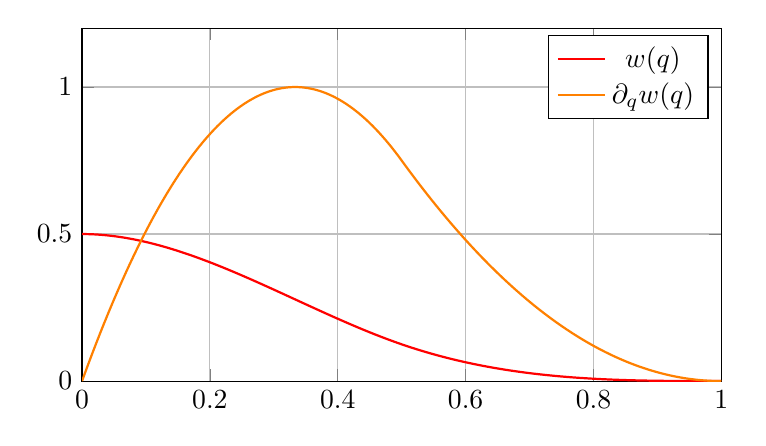
\begin{tikzpicture}[domain=0:1]
        \begin{axis}[xmin=0, xmax=1,ymin=0, ymax=1.2, grid=both,
          width=0.8\textwidth, height=0.5\textwidth]
          \addplot[red, thick, samples=100, smooth, domain=0:1]  
            {(max(0,1-\x)^3-4*max(0,0.5-\x)^3)};
          \addplot[orange, thick, samples=100, smooth, domain=0:1]  
            {(3*max(0,1-\x)^2-12*max(0,0.5-\x)^2)};
            \legend{$w(q)$, $\partial_qw(q)$,}
            \legend{$w(q)$, $\partial_qw(q)$}
        \end{axis}
      \end{tikzpicture}
      \caption{The shape function $w(q)$ that defines the Cubic Spline kernel function and its first derivative are plotted for all values of $q\in[0,1]$ that yield non-zero $w(q)$. The function is compactly supported. Since the kernel function $W$ is spherically symmetric, this one-dimensional function of the scaled distance is sufficient to describe $W$ in any dimensionality, only the scaling factors $\alpha$ have to be adjusted.}\label{fig:cubic-spline}
    \end{figure}

    \subsubsection{Differential Operators}
    The gradient of the kernel function can be used to directly to approximate differential operators such as gradient, divergence and rotation on vector fields, the least straightforward example amongst them perhaps being:
    \begin{equation}
      \angled{\nabla \vek{f}_i}_\otimes = \sum_{j\in\mathcal{N}_i} \frac{m_j}{\rho_j} \vek{f}_j \otimes \nabla W_{ij}
    \end{equation}
    where $\otimes$ is the dyadic product \autocite{tutorial2019}. Such direct discretization can lead to poor approximation quality in practice, especially for low support radii $\hbar$, which has lead to the development of alternative discretizations with useful properties.

    One such discretization is the \emphasis{difference formula}, which subtracts the first Taylor series term of the discretization error to restore 0th order consistency (see \autoref{eq:normalization-0th-order}) even for suboptimal samplings, yielding a more accurate approximation for the gradient of a scalar field \autocites{tutorial2019}{price-2012}:
    \equationnamed{Difference Formula}{\begin{equation}\label{eq:sph-difference}
      \angled{\nabla f_i}_- = \angled{\nabla f_i} - f_i\angled{\nabla 1} = \sum_{j\in\mathcal{N}_i} \frac{m_j}{\rho_j} \br{f_j - f_i} \nabla W_{ij}
    \end{equation}}

    Another useful alternative discretization for the gradient of a scalar field is the \emphasis{symmetric formula}, which can be derived from the discrete Lagrangian particularly such that when applied to the pressure field for example and a standard approximation of density is used, symmetric forces that conserve linear and angular momentum can be obtained \autocites{tutorial2019}{price-2012}:
    \equationnamed{Symmetric Formula}{
      \begin{equation}\label{eq:sph-symmetric}
        \angled{\nabla f_i}_\parallel = \rho_i\sum_{j\in\mathcal{N}_i} m_j \br{\frac{f_i}{\rho_i^2} + \frac{f_j}{\rho_j^2}} \nabla W_{ij}
      \end{equation}
    }
    While this formula is generally less accurate than the difference formula, the conservation of momenta can be a benefit that in practice outweighs lacking guarantees of first or even 0th order consistency for arbitrary samplings \autocite{tutorial2019}.

    Lastly, second derivatives must be discretized, particularly the Laplace operator necessary to describe dissipative terms such as viscosity \autocite{price-2012}. However, since the second derivative of $w(q)$ varies more intensely across the kernel support, a direct discretization would have to be exceptionally well sampled to yield accurate results - meaning the approximation quality for low support radii, sparse or high-discrepancy samplings would suffer\footnote{It might help this intuition to consider the sample positions to be quasi-randomly distributed values $X$. There exist numerous examples of upper bounds on the variance of a function of a random variable in terms of some measure of how intensely that function varies. As an example, consider random values $Z_i:=f(X_i), \mathds{V}[Z]<\infty$ in terms of some function $f:\chi\mapsto\mathds{R}$ for a measurable $\chi$ and independently distributed sample positions $X_i$ from any distribution. If $f$ has the \textit{bounded difference property} $\sup_{x'} \abs{w(x)-w(x')}\leq c$ for a non-negative bound $c$, the Efron-Stein inequality implies $\mathds{V}[Z] \leq \frac{c}{4}$ (see \cite[Boucheron et al.]{bounded-variance} for more such bounds). Since the first derivative of our shape function $\partial_qw(q)$ is more tightly bound than the second $\partial_q^2 w(q)$, achieving a lower $c$, the variance of its sampling has a tighter bound, where lower variance results in better estimator performance.}. Instead, discretizations that rely on the kernel gradient approximation are typically preferred \autocite{tutorial2019}. Amongst them, the following discretization of the Laplace operator is especially useful since for a divergence-free field $\vek{f}(\vek{x})$ it can be used to derive forces that obey momentum conservation: each summand is antisymmetric in $i,j$ and all vectorial terms are projected onto the line spanned by the positions of samples $i$ and $j$ \autocite{tutorial2019}:
    \equationnamed{Laplace Operator Discretization}{
      \begin{equation}\label{eq:sph-laplace}
        \angled{\Laplace\vek{f}_i}_\Delta = 2(d+2)\sum_{j\in\mathcal{N}_i}\frac{m_j}{\rho_j} \frac{\vek{f}_{ij}\cdot\vek{x}_{ij}}{\abs{\vek{x}_{ij}}^2}\nabla  W_{ij}
      \end{equation}
    }
    where again $d$ is the dimensionality of the problem. With this, all necessary SPH discretizations for the following chapters are available.

    \subsubsection{Particle Deficiency and Free Surfaces}\label{subsec:particle-deficiency}
    One peculiarity of the SPH discretization scheme is the behaviour at free surfaces, where the fluid phase discretized into particles meets the non-discretized phase representing for example air in a liquid simulation or vacuum in simulations of gases. Since sums over fluid particles are used to interpolate the density field $\rho$, a lack of samples in the unrepresented phase can be thought of as a perfectly dense sampling with particles that have zero density. Similarly, other field quantities such as pressure, velocity etc. are also implicitly assumed to be zero in the absence of fluid particles, which is relevant for the clamping of pressure values to positive values in \autoref{subsec:jacobi-solver}. 
    
    This leads to a phenomenon called \emphasis{particle deficiency} at the free surface, where only a section of each kernel support radius is filled with neighbouring fluid particles, leading to an underestimation of the density $\rho$ at the surface. While the implicit assumption of $\rho=0$ in the non-represented phase is not a bad assumption where $\rho_{air}\ll\rho_{H_2O}$ etc., it leads to the average density across particles $\sfrac{1}{N}\sum_i^N\rho_i$, where $\rho_i$ is SPH-discretized, depending on the geometry of the fluid, as well as always being an underestimation of the 'true' average density in the fluid. This should be accounted for when average field quantities are used, such as in the convergence criteria of pressure solvers in \autoref{subsec:iisph-convergence}.

    


\chapter{Incompressible Fluid Solver}\label{chp:fluid}
  With the SPH method from \autoref{chp:sph}, the tools to discretize and numerically solve the Navier-Stokes equations outlined in \autoref{sec:navier-stokes} are available. This chapter focuses more concretely on implementing such a fluid solver and facing the challenge of ensuring the continuity equation is upheld by an incompressible fluid. This leads to the pressure Poisson equation or PPE for short, which is iteratively solved by the Implicit Incompressible SPH solver of \autoref{sec:iisph}. Multiple source terms and variations of the solver are available, which are discussed in \autoref{sec:alternative-source-terms}.
    \section{Discretization of the Navier-Stokes Equations}\label{sec:sph-navier-stokes}
    The Navier-Stokes equations for incompressible Newtonian fluids in Lagrangian form that we consider are the continuity equation \autoref{eq:continuity} and momentum equation \autoref{eq:navier-stokes-momentum}. These form a system of equations where the momentum equation provides means of calculating the acceleration $\vek{a}_i = \frac{D\vek{v}_i}{Dt}$ necessary to compute particle trajectories using Newton's second law, while the continuity equation can be seen as a constraint on the former \autocite{tutorial2019}, ensuring incompressibility. Firstly, recall the momentum equation for some particle $i$:
    \begin{equation}\label{eq:navier-stokes-annotated}
      \underbrace{\vek{a}_i  \vphantom{\frac{1}{\rho_i}\nabla}}
        _{\text{total acceleration }}=
      \underbrace{-\frac{1}{\rho_i}\nabla p_i}
        _{\text{pressure acceleration }\vek{a}_i^p} + 
      \underbrace{\nu\Laplace\vek{v}_i  \vphantom{\frac{1}{\rho_i}\nabla}}
        _{\text{viscosity acceleration }\vek{a}_i^\nu}+
      \underbrace{\vek{b}^{ext} \vphantom{\frac{1}{\rho_i}\nabla}}
        _{\text{external accelerations eg. }\vek{g}}
    \end{equation}
    Each of these terms can now be discretized using the SPH formulas from \autoref{chp:sph}. For previously discussed reasons, the viscous term may be approximated in a symmetric and accurate fashion using the discrete Laplace operator as defined in \autoref{eq:sph-laplace}:
    \begin{equation}\label{eq:discrete-viscous}
      \angled{\nu\Laplace\vek{v}_i}_\Delta = \nu\angled{\Laplace\vek{v}_i}_\Delta = 2\nu(d+2)\sum_{j\in\mathcal{N}_i}\frac{m_j}{\rho_j} \frac{\vek{v}_{ij}\cdot\vek{x}_{ij}}{\abs{\vek{x}_{ij}}^2+\epsilon}\nabla W_{ij}
    \end{equation}
    Note the additional small term $\epsilon$ in the denominator that has been added to prevent numerical instabilities and divisions by zero if the distance between two particles was close to zero - in this implementation $\epsilon=0.01h^2$ in the expected particle spacing $h$ was chosen.
    Since viscous forces tend to be dominated by pressure forces for large-scale, low viscosity or high-Reynolds simulations as this report is subject to, the pressure acceleration is the major contributor to the particles' momenta, making the symmetric formula in \autoref{eq:sph-symmetric} a robust choice to obtain physically accurate results \autocite{tutorial2019}:
    \begin{equation}\label{eq:discrete-pressure}
      \angled{-\frac{1}{\rho_i}\nabla p_i}_\parallel 
      = -\frac{1}{\rho_i}\angled{\nabla p_i}_\parallel 
      = -\sum_{j\in\mathcal{N}_i} m_j \br{\frac{p_i}{\rho_i^2} + \frac{p_j}{\rho_j^2}} \nabla W_{ij}
    \end{equation}
    The external accelerations $\vek{b}^{ext}$ in this case are simply the gravitational acceleration $\vek{g}$ with $\abs{\vek{g}}=9.81\sfrac{\si{\meter}}{\si{\second}^2}$. 

    The density $\rho_i$ in the above approximations is a scalar quantity and can be discretized using the standard SPH sum from \autoref{eq:sph-sum} \autocite{tutorial2019}:
    \begin{align}\label{eq:discrete-density}
      \angled{\rho_i}  
      = \sum_{j\in\mathcal{N}_i} \frac{m_j}{\rho_j} \rho_j W_{ij} 
      = \sum_{j\in\mathcal{N}_i} m_j W_{ij} 
    \end{align}

    Since the mass $m_i$ is set at the start of the simulation, $\nu,\vek{g}$ are given and initial $\vek{x}_i, \vek{v}_i$ are known, the only quantity in the momentum equation yet to be accounted for is the pressure field $p$. The system could be closed by employing a state equation relating the pressure directly to the density field using some stiffness parameter $k$ through the ideal gas equation $p=k\rho$ \autocite{müller-2003}, the Murnaghan equation of state \autocite{murnaghan-eos} as used in Weakly Compressible SPH \autocite{wcsph} $p=k\br{\br{\sfrac{\rho}{\rho_0}}^\gamma-1}$ or similar equations of state. Since for the incompressible fluids simulated in this report the constraints imposed by the continuity equation must be strongly enforced, pressure is instead computed iteratively by solving a pressure Poisson equation or PPE as outlined in \autoref{sec:iisph}.

    In the following, quantities $f_i$ will generally refer to the SPH-discretized fields for brevity.

    \subsubsection{Time Discretization}
    After spatial discretization using the SPH scheme, the second order partial differential equation \autoref{eq:navier-stokes-momentum} is turned into an ordinary differential equation \autocite{tutorial2019} that must be discretized in time. 
    % Equipped with an initial state $\{\forall i:\br{\vek{x}_i(t_0),\vek{v}_i(t_0),m_i(t_0)}\}$ that is assumed to be a valid state of the fluid, as well as the discrete momentum equation to calculate accelerations $\vek{a}_i(t)$ with, numerical time integration schemes can be used to solve the equation of motion and propagate the solution forwards in time.

    For this purpose, time is discretized into time steps $\Delta t$ and a numerical integration scheme is applied to obtain particle trajectories by updating particle positions and velocities. In Computer Graphics literature, the most prevalent scheme \autocites{tutorial2019}{wcsph}{iisph}{iisph-flip}{dfsph} to this end is symplectic or semi-implicit Euler time integration:
    \begin{align}\label{eq:numerical-time-integration}
      \vek{v}(t+\Delta t) &= \vek{v}(t) + \Delta t \vek{a}(t)\\
      \vek{x}(t+\Delta t) &= \vek{x}(t) + \Delta t \vek{v}(t+\Delta t)
    \end{align}

    There is a trade-off in choosing a time step size: large time steps mean more progress per solver step and can lead to greater efficiency, while time steps that are too large might lead to instability and can actually cause lower overall performance especially for iterative solvers, as will be discussed later. A common upper bound on $\Delta t$ is the Courant-Friedrichs-Lewy or CFL condition, which states that particles should not move further than some fraction $\lambda\in\left]0,1\right]$ of their size or spacing $h$ within one time step, which for a global adaptive time step size implies \autocite{tutorial2019}:
    \begin{equation}\label{eq:cfl-condition}
      \Delta t \leq \lambda \frac{h}{\max_i \abs{\vek{v}_i}}
    \end{equation}
    with a common choice \autocites{dfsph}{monaghan92} being $\lambda=0.4$. Alternative formulations based on the maximum accelerating forces \autocites{monaghan92}{time-adaptive-sph} or more elaborately derived formulas that differ per kernel function and pressure solver \autocite{optimal-timestep} exist.


    \subsubsection{Initial conditions}\label{subsec:initial-conditions}
    The numerical time integration scheme propagates a solution to the governing equations forwards in time, calculating a new valid state of the fluid at $t+\Delta t$ from a current one at time $t$. To seed this recursion, an initial state at $t_0$ must be provided. Perhaps the simplest and most common method of creating such an initial state is to define a volume filled with liquid in the simulation domain and sample it with fluid particles on a regular, square grid with spacing $h$, initial zero velocities, and a uniform rest volume $V_0=\sfrac{1}{h^d}$, or equivalently mass $m_0 = \sfrac{\rho_0 }{h^d}$ in $d$ dimensions. This method poses two challenges in particular: one is sampling an arbitrary fluid volume, the other is preventing artefacts due to the anisotropic, regular sampling and ensuring that the initial stages of the simulation run smoothly. 

    \begin{itemize}
      \item  The first problem of sampling some closed volume with fluid particles is trivial when that volume is a box. More generally, a watertight mesh that bounds the fluid volume can be provided, where candidate fluid particle positions are sampled on a regular grid of spacing $h$ within the axis-aligned bounding box of said mesh. For each such candidate position, since the mesh is watertight, a single ray cast operation is sufficient to determine whether the position is within the fluid volume or not: according to the Jordan Curve theorem, if any ray originating at the candidate position intersects the bounding mesh an odd number of times, the point lies within the volume \autocite{point-in-polygon} and a fluid particle is instantiated, otherwise the candidate is discarded\footnote{The implementation of this report uses the \texttt{trimesh.ray.ray\_pyembree.RayMeshIntersector} implementation of a ray cast operator \autocite{trimesh}}. Additionally, all candidate positions closer than $h$ to a boundary particle as described in \autoref{sec:boundary} can be discarded to prevent boundary penetration and unnaturally high pressure values at $t_0$.
      \item The second problem may be alleviated by applying a jitter on initial positions in conjunction with non-uniform particle masses \autocite{labcourse}. Sampling particles of uniform mass causes a density gradient due to particle deficiency towards the boundary of the fluid volume, which can in turn result in an erroneous pressure gradient that causes the fluid to expand towards the boundary, causing an 'explosion'. The mass of each particle can instead be chosen such that uniform rest density $\rho_0$ is achieved everywhere at $t_0$ by assigning a higher rest volume to particles at boundaries, ensuring $\forall i: \rho_i(t_0)=\rho_0\Longrightarrow p_i(t_0)=0$. It is easy to see that this can be implemented in a manner consistent with the employed SPH density approximation by iterating:
      \item \begin{align}
        m_i^0 &= \frac{1}{h^d}\\
        \angled{\rho_i}^l &\gets \sum_{j\in\mathcal{N}_i} m_j^l W_{ij} \\
        m_i^{l+1} &\gets m_i^l \cdot \frac{\rho_0}{\angled{\rho_i}^l}\label{eq:initializing-fluid-rest-density}
      \end{align}
      until convergence, which in this implementation was defined as when the average density error $\frac{1}{N}\sum_{i}\rho_i - \rho_0$ changes by less than $10^{-10}\frac{\si{\kg}}{\si{\meter}^3}$ compared to the previous iteration. Stricter bounds are unproblematic since the cost is a one-off preprocessing computation. Slow convergence can be seen as an indicator for an ill-defined scene specification. 

      This initialization to rest density enables another possible improvement in the form of jittered initial positions. A regular grid in conjunction with a kernel with support radius $\hbar$ that is an integer multiple of the grid spacing $h$ was found to be exceptionally prone to aliasing artefacts in the initial stages of simulation. Even just a jitter of $\overrightarrow{\Delta x} \sim 0.01h\cdot\mathcal{N}\br{\vek{\mu}=\vek{0}, \vek{\sigma}=\vek{1}}$ was found in this implementation to relieve numerical issues and anisotropic behaviour, while the uniform density initialization prevents the jitter from resulting in erroneous initial pressure forces. Slightly non-uniform particle masses are also suspected to persistently improve the amorphousness of the particle sampling, reducing numerical viscosity \autocite{labcourse}.
    \end{itemize}
   

    \section{The Pressure Poisson equation}
    With the discretization of the Navier-Stokes equations from \autoref{sec:sph-navier-stokes}, a simple equation-of-state based solver such as Weakly Compressible SPH or WCSPH for short, could be implemented directly. However, such a solver that computes pressure accelerations at particles only locally, from immediately neighbouring particles at each time step, can exhibit noticeable oscillations as the complexity of the scene, namely the maximum height of a column of fluid supported by the pressure, increases.

    As such a column of particles is uniformly accelerated by gravity but faces an impenetrable boundary at its bottom, a counteracting pressure gradient has to build up. Since pressure is only computed locally and the numerical speed of sound is low, particles will continue to fall, increasing measured density and thereby pressure beyond the linear gradient necessary to counteract gravity, until this superlinear gradient pushes the top of the column up beyond its hydrostatic resting position and repeating, resulting in unrealistic oscillations. In other words, it is hard to enforce incompressibility with such a solver: even if a large stiffness coefficient $k$ is chosen to counteract this effect and increase the numerical speed of sound, a correspondingly small time step size $\Delta t$ would be required to keep the system numerically stable, decreasing efficiency \autocite{iisph}. 
    
    Alternatively, the differential density deviation $\frac{D}{Dt}\rho$ could be penalized, however while no oscillations would occur, numerical errors would instead accumulate into volume drift \autocite{tutorial2019}, leading to arguably worse results where the fluid volume would irrecoverably decrease over time and accurate boundary conditions are challenging to implement. The misconception that volume oscillations are inherent to Lagrangian methods such as SPH fluid simulation can instead be interpreted as a deliberate choice enabling accurate simulation of free-surface flows where volume drift would lead to noticeable errors.
  
    To tackle this issue, the solution of the Navier-Stokes equation can be decomposed into sequential sub-problems, namely into pressure accelerations and non-pressure accelerations such as caused by gravity and viscosity \autocite{tutorial2019}. The idea is to integrate the less problematic sub-problem explicitly, while the dominating pressure accelerations can subsequently be implicitly determined to leave the fluid in a divergence-free or uncompressed predicted state at the next time step \autocite{tutorial2019}. This is also referred to as \emphasis{operator splitting} \autocite{tutorial2019} and implemented here as computing the predicted velocity $\vek{v}_i^*$ due to non-pressure accelerations:
    \begin{align}
      \vek{v}_i^*\br{t} = \vek{v}\br{t} + \Delta t\br{\vek{g} + \nu\Laplace\vek{v}_i\br{t}}\label{eq:operator-splitting}
    \end{align}
    before implicitly integrating the pressure acceleration $\vek{a}_i^p$ as described in \autoref{sec:iisph}. This equates to solving the \emphasis{Pressure Poisson equation}, or PPE for short, which will be derived and discretized in the following and is used to project the particle velocities onto an uncompressed or divergence-free state.

    \subsubsection{Derivation of the Pressure Poisson Equation}

    Pressure computation is, in the case of inviscid flows, the stiff sub-problem in the partial differential equations to solve \autocite{tutorial2019}. Pressure values that strongly enforce incompressibility, or in other words act as Lagrange multipliers to the continuity equation \autoref{eq:continuity} \autocite{tutorial2019}, should be computed efficiently. This can be done using iterative, global solvers that solve the Pressure Poisson equation, which asserts that the pressure forces do in fact enforce the continuity equation. 
    
    One way to derive the PPE is to focus on the density invariance constraint imposed by the continuity equation (see constraint \ref{enum:continuity-equation-constraint-den}). A predicted velocity $\vek{v}_i^*$ would result in positions $\vek{x}_i^*$ that can be used to compute a predicted density $\rho_i^*$ using, for example, \autoref{eq:discrete-density-boundary}. The incompressibility constraint then means that:
    \begin{equation}\label{eq:ppe-incompressibility-constraint}
      \forall i: \rho_i\br{t+\Delta t}=\rho_0
    \end{equation} 
    must hold, or that the pressure acceleration must cause a change to the predicted density that keeps the measured density $\rho_i\br{t+\Delta t}$ at the next time step at the rest density everywhere.
    
    Updating particle positions to $\vek{x}_i^*$ in a sub-step, recomputing the sets of neighbours that depend on those positions and using \autoref{eq:discrete-density-boundary} to compute $\rho_i^*$ is not done in practice, since the recalculation of neighbours is computationally expensive. Instead, the predicted density can be obtained by numerically integrating the change in density $\br{\sfrac{D\rho}{Dt}}^*$ due to $\vek{v}_i^*$ to estimate the density at the next time step \autocite{tutorial2019}:
    \begin{align}
      \rho^* &= \rho + \Delta t \br{\frac{D\rho}{D t}}^* &\textit{approximate density at next time step}\\
      \rho^*&=\rho + \Delta t \br{-\rho\divergence\vek{v}^*} &\textit{insert continuity equation \ref{eq:continuity}}\\
      \rho^* &= \rho - \Delta t \rho \divergence \vek{v}^* \label{eq:ppe-rho-star}
    \end{align}

    \autoref{eq:ppe-rho-star} encodes the fact that a velocity field with negative divergence at a point will see an increase in density, while positive divergence of the velocity field means a decrease in mass density. 

    This same formula can be used to predict a density change $\rho_p^*$ due to the pressure acceleration:
    \begin{align}
      \rho_p^* &= \rho - \Delta t \rho \divergence \br{\Delta t\vek{a}_p} &\textit{\autoref{eq:ppe-rho-star} using $\vek{v}^*_p = \Delta t \vek{a}_p$ instead of $\vek{v}^*$}\\
      &= \rho - \Delta t \rho \divergence \br{\Delta t\br{-\frac{1}{\rho}\nabla p}} &\textit{Definition of $\vek{a}_p$ from \autoref{eq:navier-stokes-annotated}}\\
      &= \rho + \Delta t^2 \divergence \br{\nabla p} &\textit{simplify}\\
      \rho_p^* &= \rho + \Delta t^2 \Laplace p &\textit{$\divergence \br{\nabla p} = \Laplace p$}\label{eq:ppe-rho-star-prs}
    \end{align}
    Finally, one can assert that adding the predicted change in density due to the pressure acceleration $\rho_p^* - \rho$ to the predicted density due to non-pressure accelerations $\rho^*$ should result in rest density $\rho_0$ at the next time step:
    \begin{align}
      \rho\br{t+\Delta t} &\overset{!}{=} \rho_0 &\textit{incompressibility constraint \autoref{enum:continuity-equation-constraint-den}, \autoref{eq:ppe-incompressibility-constraint}}\\
      \rho^* + \br{\rho_p^* - \rho} &\overset{!}{=} \rho_0 &\\
      \rho^* \cancel{+ \rho} + \Delta t^2 \Laplace p \cancel{- \rho} &\overset{!}{=} \rho_0 &\textit{insert \autoref{eq:ppe-rho-star-prs}}\\
      \Delta t \Laplace p &\overset{!}{=}\frac{\rho_0-\rho^*}{\Delta t} &\textit{rearrange}
    \end{align}
    which is one form of the pressure Poisson equation \autocite{tutorial2019}. 
    Basically the exact same derivation can be used with constraint \ref{enum:continuity-equation-constraint-vel} derived from the continuity equation, namely a divergence free velocity field at the next time step. Note the similarity to the derivation above:
    \begin{align}
      \divergence\br{\vek{v}\br{t+\Delta t}} &\overset{!}{=} 0&\textit{divergence free velocity constraint \ref{enum:continuity-equation-constraint-vel}}\\
      \divergence\br{\vek{v}^* - \Delta t \frac{1}{\rho}\nabla p} &\overset{!}{=} 0 &\textit{insert $\vek{v}_p^*=\Delta t \br{- \frac{1}{\rho}\nabla p}$}\\
      \divergence\vek{v}^* - \Delta t \frac{1}{\rho}\Laplace p &\overset{!}{=} 0 & \textit{linearity of divergence}\\
      \Delta t \Laplace p&\overset{!}{=} \rho \divergence\vek{v}^* &\textit{rearrange}
    \end{align}

    
    \subsubsection{Discretizing the Pressure Poisson Equation}
    The focus in the following lies on the density invariance source term, or in other words discretizing the PPE:
    \begin{equation}
      \Delta t^2 \Laplace p = \rho_0-\rho^*
    \end{equation}
    using the SPH scheme so that it can be solved numerically at each discrete particle location.

    For this purpose, the following discretization of the divergence of a vector field, derived from the standard SPH sum (\autoref{eq:sph-sum}) by pulling the density into the differential operator, is commonly employed \autocites{monaghan92}{2014-survey-state-of-the-art-sph}: 
    \begin{align}
      \divergence \vek{f}&= \frac{1}{\rho}\br{\divergence \br{\vek{f}\rho} - \vek{f}\cdot\nabla\rho}
      &\textit{after \autocite[Monaghan 1992]{monaghan92}}\\
      \angled{\divergence \vek{f}} &= \frac{1}{\rho_i} \underbrace{\sum_{j\in\mathcal{N}_i}  \frac{m_j}{\rho_j} \br{\rho_j\vek{f}_j} \cdot \nabla W_{ij}}_{\angled{\divergence \br{\vek{f}\rho}}}
        - \frac{1}{\rho_i} \underbrace{\vek{f}_i \cdot \sum_{j\in\mathcal{N}_i}  m_j \nabla W_{ij}}_{\vek{f}_i\cdot \angled{\nabla\rho}}&\textit{SPH sum (\autoref{eq:sph-sum})}
    \end{align}
    which simplifies to:
    \equationnamed{SPH divergence discretization}{
      \begin{equation}
        \angled{\divergence \vek{f}}_{\divergence} = 
        -\frac{1}{\rho_i} \sum_{j\in\mathcal{N}_i}  
          m_j\vek{f}_{ij}\cdot\nabla W_{ij}
        \label{eq:sph-divergence}
      \end{equation}  
    }

    Using this, the source term $s_i=\rho_0-\rho^*_i$ can be discretized as:
    \begin{align}
      \angled{\rho_0-\rho^*} &= \rho_0 - \br{\rho_i - \Delta t \rho_i \angled{\divergence \vek{v}^*_i}_\divergence} &\textit{Definition of $\rho^*$ (\autoref{eq:ppe-rho-star})}\\
      &= \rho_0 - \br{\rho_i + \Delta t \cancel{\rho_i} \br{\cancel{\frac{1}{\rho_i}} \sum_{j\in\mathcal{N}_i} m_j\vek{v}^*_{ij}\cdot\nabla W_{ij}}} &\textit{apply $\divergence$ discretization (\autoref{eq:sph-divergence})}\\
      &= \rho_0 - \rho_i - \Delta t \sum_{j\in\mathcal{N}_i}  m_j\vek{v}^*_{ij}\cdot\nabla W_{ij} &\textit{simplify}
    \end{align}
    which can be extended using the boundary handling of \autoref{chp:rigid} like in \autoref{subsub:bdy-extend-governing} to:
    \begin{equation}
      s_i = \angled{\rho_0-\rho^*} =
      \rho_0 - \rho_i 
      - \Delta t \sum_{j\in\mathcal{N}_i}  m_j\vek{v}^*_{ij}\cdot\nabla W_{ij} 
      - \Delta t \sum_{k\in\mathcal{B}_i}  m_k\vek{v}^*_{ik}\cdot\nabla W_{ik}
      \label{eq:iisph-source-term}
    \end{equation}
    where for static boundaries one can assume $\vek{v}^*_k=\vek{0}$ while for weakly coupled dynamic rigid bodies as describe in \autoref{sec:rigid-bodies} $\vek{v}^*_k \approx \vek{v}_k\br{t}$ can serve as a best guess approximation. 
    
    \horizontalspacer

    Secondly, the term $\Delta t^2\Laplace p$ needs to be discretized. To this end, a discretization consistent with the computation of the pressure acceleration in \autoref{eq:discrete-pressure-bdy} should be chosen, such that the solver computes pressures that actually translate to the predicted, uncompressed state after $\vek{a}_i^p$ has been computed from each $p_i$ \autocite{tutorial2019}:
    \begin{align}
      \angled{\Delta t^2\divergence\br{\nabla p}} &= \Delta t^2\angled{\divergence\br{-\rho_i \vek{a}_i^p}}_\divergence &\textit{since $ \vek{a}_i^p=-\frac{1}{\rho_i}\nabla p$ (\autoref{eq:navier-stokes-annotated})}\\
      &= - \rho_i \Delta t^2\angled{\divergence\br{\vek{a}_i^p}}_\divergence&\textit{use linearity}\\
      &= 
      \Delta t^2 \sum_{j\in\mathcal{N}_i} m_j \vek{a}^p_{ij} \cdot \nabla W_{ij}
      &\textit{apply $\divergence$ discretization (\autoref{eq:sph-divergence})}
    \end{align}
    which extends when considering boundary particles to a term:
    \begin{equation}
      \angled{\Delta t^2\divergence\br{\nabla p}} =
      \Delta t^2 \sum_{j\in\mathcal{N}_i} m_j \vek{a}^p_{ij} \cdot \nabla W_{ij}
      +\Delta t^2 \sum_{k\in\mathcal{B}_i} m_k \vek{a}^p_{i} \cdot \nabla W_{ik}\label{eq:iisph-ap_i}
    \end{equation}
    with the simplifying assumption that pressure accelerations $\vek{a}^p_k$ at boundary particles are zero. 
    
    Note that the discretization of the Laplace operator $\Laplace p$ using the discretization of the divergence in $\angled{\divergence\br{\nabla p}}$ is not the only possibility, and other discretizations such as the discrete Laplace operator in \autoref{eq:sph-laplace} commonly used to compute viscosities, is also thinkable. For one comparison of the discretization used in \autocite[Implicit Incompressible SPH]{iisph}, which is presented here, to \autoref{eq:sph-laplace} we refer to \autocite[Fürstenau et al.]{fuerstenau-laplace-discretization-comparison}.
    
    \section{Implicit Incompressible SPH}\label{sec:iisph}
    With the discretized pressure Poisson equation obtained, one can go about solving the resulting system of $N$ equations at $N$ particles for the unknown pressure values $p_i$. Many possible solvers for this problem exist, such as Conjugate-Gradient \autocite[as alternatively proposed by Ihmsen et al.]{iisph}, and more recently Nonsmooth Nonlinear Conjugate Gradient methods as suggested by \autocite[Probst and Teschner]{monolithic-rigids-timo}.

    A relatively straightforward implementation that is robust, matrix-free, i.e. does not rely on explicitly constructing system matrices of prohibitive $\mathcal{O}\br{N^2}$ proportions, and which can be fully parallelized is achieved by a \emphasis{Relaxed Jacobi Solver} as suggested in Implicit Incompressible SPH or IISPH for short \autocite[by Ihmsen et al.]{iisph}. 

    When using relaxed Jacobi iterations, the system of $N$ equations:
    \begin{equation}
      \mathds{A}\vek{p} = \vek{s}
    \end{equation}
    can be solved using only the product $\br{\mathds{A}\vek{p}}_i$ on the left-hand side for each particle, which is exactly \autoref{eq:iisph-ap_i}, and the diagonal element $\mathds{A}_{ii}$ of the $N\times N$ matrix $\mathds{A}$ which encodes the Laplace operator and the double integration with respect to time. The diagonal elements are can be thought of as the coefficients of $p_i$ in the $i$-th equation of $\br{\mathds{A}\vek{p}}_i$ (which is \autoref{eq:iisph-ap_i}) - the plan in the following is to write out that $i$-th expression explicitly and factor out all the coefficients of $p_i$ within it, starting with the pressure acceleration:
    \begin{align}
      \vek{a}_i^p &= -
      \sum_{j\in\mathcal{N}_i} 
        m_j \br{\frac{p_i}{\rho_i^2} + \frac{p_j}{\rho_j^2}} \nabla W_{ij} 
      -\sum_{k\in\mathcal{B}_i} 
        m_k\frac{p_i}{\rho_i^2} \nabla W_{ik} 
      &\textit{\autoref{eq:discrete-pressure-bdy}}\\
      &= p_i \underbrace{\frac{1}{\rho_i^2}\br{
        -\sum_{j\in\mathcal{N}_i} 
        m_j \nabla W_{ij} 
        -\sum_{k\in\mathcal{B}_i} 
        m_k \nabla W_{ik} 
      }}_{=: \vek{c}_i}
      - \sum_{j\in\mathcal{N}_i} 
        m_j\frac{p_j}{\rho_j^2} \nabla W_{ij} 
      &\textit{factor out $p_i, \sfrac{1}{\rho_i^2}$}
      % &= p_i \vek{c}_i - \sum_{j\in\mathcal{N}_i\setminus\{i\}} 
      %   m_j\frac{p_j}{\rho_i^2} \nabla W_{ij} 
      % &\textit{$\nabla W_{ii}=0$ due to \autoref{eq:sph-property-symmetry}}
    \end{align}
    where since the kernel is spherically symmetric (\autoref{eq:sph-property-symmetry}) and differentiable and therefore $\nabla W_{ii}=0$ holds, one can exclude the index $i$ from the set of neighbours and write:
    \begin{align}
      \vek{a}_i^p &= p_i \vek{c}_i - 
      \sum_{j\in\mathcal{N}_i\setminus\{i\}} 
        m_j\frac{p_j}{\rho_j^2} \nabla W_{ij} \label{eq:iisph-a-p-c_i}
    \end{align}
    which makes it easier to extract the $p_i$ in the larger expression $\br{\mathds{A}\vek{p}}_{i}$ as follows:
    \begin{align}
      \br{\mathds{A}\vek{p}}_{i}
      ={}&\Delta t^2 \sum_{j\in\mathcal{N}_i} m_j \vek{a}^p_{ij} \cdot \nabla W_{ij}
      +\Delta t^2 \sum_{k\in\mathcal{B}_i} m_k \vek{a}^p_{i} \cdot \nabla W_{ik} 
      &\textit{\autoref{eq:iisph-ap_i}}\\
      \begin{split}
        ={}&\Delta t^2 \sum_{j\in\mathcal{N}_i} m_j \vek{a}^p_{i} \cdot \nabla W_{ij}
        -\Delta t^2 \sum_{j\in\mathcal{N}_i} m_j \vek{a}^p_{j} \cdot \nabla W_{ij}\\
        &+\Delta t^2 \sum_{k\in\mathcal{B}_i} m_k \vek{a}^p_{i} \cdot \nabla W_{ik}
      \end{split}
      &\textit{split $\vek{a}^p_{ij}$}
    \end{align}
    Inserting \autoref{eq:iisph-a-p-c_i} for $\vek{a}_i^p, \vek{a}_j^p$ then yields:
    \begin{align*}
      \br{\mathds{A}\vek{p}}_{i}={}
        &\Delta t^2 \sum_{j\in\mathcal{N}_i} m_j 
         \br{p_i \vek{c}_i 
         \underbrace{- \sum_{j\in\mathcal{N}_i\setminus\{i\}} m_j\frac{p_j}{\rho_j^2} \nabla W_{ij}}_{\textit{does not contribute, $j\neq i$}}
         } 
         \cdot \nabla W_{ij}
         &\textit{insert \autoref{eq:iisph-a-p-c_i}}\\
       &-\Delta t^2 \sum_{j\in\mathcal{N}_i} m_j 
         \br{
           \underbrace{p_j \vek{c}_j}_{\textit{no contribution for $i=j$ since $\nabla W_{ii}=0$}}
           \underbrace{- \sum_{l\in\mathcal{N}_j\setminus\{j\}} m_l\frac{p_l}{\rho_l^2} \nabla W_{jl}}_{\textit{only contributes for $l=i$}}
         }
         \cdot \nabla W_{ij}
         &{}\\
       % &-\Delta t^2 \sum_{j\in\mathcal{N}_i} m_j \br{\vek{a}^p_{j}} \cdot \nabla W_{ij}\\
       &+\Delta t^2 \sum_{k\in\mathcal{B}_i} m_k 
         \br{p_i \vek{c}_i 
           \underbrace{- \sum_{j\in\mathcal{N}_i\setminus\{i\}} m_j\frac{p_j}{\rho_j^2} \nabla W_{ij}}_{\textit{does not contribute, $j\neq i$}}
         } 
         \cdot \nabla W_{ik}
         &{}
    \end{align*}
    Note here that the index $l$ refers to the neighbours of the neighbours of particle $i$. Exactly one of these second-degree neighbours $l$ refers back to $i=l$ and therefore contains a $p_i$ that contributes to $\mathds{A}_{ii}$, all other terms in the sum are irrelevant. Also note that sums over $\mathcal{N}_i\setminus\{i\}$ explicitly do \textit{not} contain the term $p_i$ and can therefore be completely ignored. With $\br{\mathds{A}\vek{p}}_i$ in a form that allows all coefficients of $p_i$ in the $i$-th equation of the system to be extracted, the diagonal element $\mathds{A}_{ii}$ can be obtained by taking the partial derivative with respect to $p_i$, resulting in:
    \equationnamed{Diagonal Element $\mathds{A}_{ii}$}{
      \begin{align}
        \begin{split}
          \mathds{A}_{ii} = \frac{\partial \br{\mathds{A}\vek{p}}_i}{\partial p_i} &=\Delta t^2\sum_{j\in\mathcal{N}_i} m_j \vek{c}_i \cdot \nabla W_{ij}\\
          &+ \Delta t^2 \sum_{j\in\mathcal{N}_i} m_j \br{
             \frac{m_i}{\rho_i^2}\nabla W_{ji}
          } \cdot \nabla W_{ij}\\
          &+\Delta t^2 \sum_{k\in\mathcal{B}_i} m_k 
            \vek{c}_i
          \cdot \nabla W_{ik}
        \end{split}\label{eq:iisph-diagonal-element}\\
        \textit{where: \quad}\vek{c}_i &:= \frac{1}{\rho_i^2}\br{-\sum_{j\in\mathcal{N}_i} 
        m_j \nabla W_{ij} 
       -\sum_{k\in\mathcal{B}_i} 
        m_k \nabla W_{ik} }
      \end{align}
    }
    
    The diagonal element depends only on the current positions, neighbour sets, masses and densities of the particles, all of which do not change within the simulation step, meaning the diagonal element can be computed once per time step after the density has been computed and then reused in each iteration of the iterative solver described in the following. 
    
    It is also worth noting that both the specific boundary handling method described in \autoref{chp:rigid}, namely \autocite[consistent boundaries]{consistent-boundaries} with density mirroring, as well as the semi-implicit time integration scheme used in \autoref{eq:numerical-time-integration} and the operator splitting in \autoref{eq:operator-splitting} are used in the derivation of the expression for $\mathds{A}_{ii}$ and the diagonal element needs to be adjusted if any of these components differ.

    Lastly, a slight variation of the algorithm was implemented based on the assumption that for strongly enforced incompressibility $\rho_i=\rho_j=\rho_0$ holds, namely all densities in the pressure solver and the pressure acceleration calculation were replaced with $\rho_0$. This not only allows a lot of refactoring of the terms for greater efficiency with fewer read operations to memory, but was hoped to result in a more robust solver. 

    \subsubsection{Relaxed Jacobi Solver}\label{subsec:jacobi-solver}
    With the source term $s_i$ shown in \autoref{eq:iisph-source-term}, the diagonal element $\mathds{A}_{ii}$ from \autoref{eq:iisph-diagonal-element}, both of which can be pre-computed, as well as the pressure acceleration $\vek{a}_i^p$ in \autoref{eq:discrete-pressure-bdy} and the right-hand side of the PPE $\br{\mathds{A}\vek{p}}_i$ in \autoref{eq:iisph-ap_i}, all the values required to implement a relaxed Jacobi solver and solve the system of equations for the unknown pressures $p_i$ are available. The core idea here is to iterate:
    \begin{equation}
      p_i^{l+1} = \br{p_i^{l} + \omega \frac{s_i-\br{\mathds{A}\vek{p}_i}}{\mathds{A}_{ii}}\cdot\mathds{1}\br{\mathds{A}_{ii}>\epsilon}}_+\label{eq:iisph-relaxed-jacobi-iteration}
    \end{equation}
    until the predicted density error per particle $\br{\rho^{err}_i}^l = \br{\mathds{A}\vek{p}}_i-s_i$ fulfils some convergence criterion. The indicator function $\mathds{1}\br{P}$ for a predicate $P$ is used to only update the pressure when the diagonal element, which the predicted density error is divided by, is greater than some positive, small threshold like $\epsilon=10^{-6}$ in order to avoid numerical instabilities and divisions by zero. Note also the use of the clamping operator $\br{x}_+ = \max\br{0, x}$ that can be viewed as a proximal operator \autocite{monolithic-rigids-timo} and ensures that pressure values are always positive. This prevents undesirable clumping artefacts that could otherwise occur when using an SPH discretization \autocite{iisph} and are speculated to result from the assumption that regions with incompletely sampled regions at free surfaces are implicitly assumed to have a pressure value of zero where there are no fluid particles \autocite{tutorial2019}. Since the solver is run until convergence, this clamping is unproblematic because it effectively shifts all pressure values up to be positive, while not changing the pressure \textit{gradient} that is actually used to compute pressure forces and accelerations \autocite{tutorial2019}.

    The choice of relaxation parameter $\omega\in\left]0,1\right[$ is not just the namesake of the relaxed Jacobi solver but determines its convergence properties: like with any relaxation scheme, a higher value of $\omega$ leads to faster convergence, while a lower value of $\omega$ might prevent numerical instabilities. In practice, the critical value $\omega=0.5$ is used, which is the highest value that has been shown to lead to robust convergence \autocite{iisph}.

    For the initial iteration $l=0$, the authors of the \autocite[original paper]{iisph} recommend warm-starting the solver by initializing all pressure values $\vek{p}$ with half the pressure computed in the previous time step, i.e.:
    \begin{equation}
      p^0_i\br{t} = \omega_{warm}p^0_i\br{t-\Delta t_{prev}}
    \end{equation}
    with $\omega_{warm}=0.5$. Since the initial time step $t=0$ ought to be an uncompressed state anyways, the base case of this backwards recursion is unproblematic. However, a more conservative initialization using $\omega_{warm}=0$, which realizes a cold start of the solver, can be used instead to trade off some performance for more robust behaviour. The relaxed Jacobi solver as presented in \autoref{eq:iisph-relaxed-jacobi-iteration} can suffer in practice from divergence and in consequence exploding pressure values when the initial guess for the pressures $p_i^0$ is too high, so for especially complex scenes with high fluid columns and where pressures might change abruptly, cold-starting the solver might be preferable when a slightly higher iteration count per time step can be tolerated.


  \subsubsection{Convergence Criteria}\label{subsec:iisph-convergence}
  The Jacobi iteration in \autoref{eq:iisph-relaxed-jacobi-iteration} is repeated until the pressure values $p_i$ have converged to a solution that ensures incompressibility at the next time step, but the exact stopping criterion or convergence criterion has yet to be discussed. 

  In \autoref{subsec:jacobi-solver} the predicted density error $\br{\rho^{err}_i}^l = \br{\mathds{A}\vek{p}}_i-s_i$ that appears in the Jacobi update has already been mentioned. This predicted error is not exactly equal to the density error at the next time step since some approximations were made, for example when a repeated neighbourhood search was foregone in favour of calculating predicted density $\rho^*$ using the velocity divergence in \autoref{eq:ppe-rho-star}. However, the predicted density error is, by design, as close as possible to the actual density error at the next time step as can be, given the information available, and can be reused from \autoref{eq:iisph-relaxed-jacobi-iteration} at no additional computational cost, so it is often used \autocites{tutorial2019}{iisph}. 

  Two predicted error metrics are commonly employed \autocite{iisph}:
  \begin{align}
    \rho^{l}_{max} &= \frac{1}{\rho_0}\max\br{\{\forall i\in\mathcal{N}_1^N: \br{\rho^{err}_i}^l\}} 
    &\textit{Maximum predicted density error}\\
    \rho^{l}_{avg} &= \frac{1}{\rho_0}\frac{1}{N}\sum_{i=1}^N \br{\rho^{err}_i}^l
    &\textit{Average predicted density error}
  \end{align}

  The \autocite[authors of IISPH]{iisph} recommend iterating until the average predicted density error is below a threshold of $0.1\%$, such that no oscillations in the fluid are perceptible. The ratio of $\rho^{l}_{max}$ and $\rho^{l}_{avg}$ varies, so the authors argue that the keeping the maximum error fixed does not prevent visual artefacts that stem from varying average density, especially for tall fluid columns in complex scenes \autocite{iisph}. 
  
  On the other hand, recalling the particle deficiency phenomenon discussed in \autoref{subsec:particle-deficiency}, the average density can inadvertently be influenced by the geometry of the fluid, where a fluid with a large surface area and therefore many particles at the free surface can have its 'true' average density underestimated by the SPH discretization. This was found in this implementation to negatively impact simulations of, for example, shallow waters, where the solver might stop iterating prematurely because of this underestimation of average density. The maximum density metric does not suffer from this issue, so a conjunction of both convergence criteria was used in the implementation presented here to achieve more robust behaviour for arbitrary scenes. 

  Note that the maximum predicted density error is a strict upper bound of the average predicted error, so the threshold for $\rho^{l}_{max}$ poses a stricter constraint and can be relaxed to $0.5\%$ for example.

  The final convergence criterion is a boolean predicate on the predicted density errors $\br{\rho_i^{err}}^l$ in the $l$-th iteration and can be stated as:
  \begin{equation}
    \br{\rho^l_{avg} \leq \rho^{thresh}_{avg}}
    \land \br{\rho^l_{max} \leq \rho^{thresh}_{max}}
    \land \br{l_{min} \leq l \leq l_{max}}
    \label{eq:convergence-criterion}
  \end{equation}
  where minimum and maximum solver iteration counts such as $l_{min}=3, l_{max}=\infty$ can be added to increase robustness and ensure reasonably converged pressure values to use when warm-starting the next iteration. Recommended choices for the threshold values are $\rho^{thresh}_{avg}=0.1\%$ \autocite{iisph} and $\rho^{thresh}_{max}=0.5\%$.

  Using only upper bounds as thresholds, i.e. $\leq$ in \autoref{eq:convergence-criterion}, ensures that only compressions are penalized by the solver whereas a predicted density below rest density is allowed, since the particle deficiency phenomenon (see \autoref{subsec:particle-deficiency}) could otherwise cause the solver to never converge when the ratio of surface area to volume of the fluid in its current configuration is large and for example $\abs{\rho^l_{avg}} \leq \rho^{thresh}_{avg}$ would never be true. 

  % This means that technically, the lowest pressure values that satisfy the convergence predicate should be obtained by the solver, but arbitrarily larger pressure values that cause an explosion of the fluid could also satisfy the convergence criterion \autoref{eq:convergence-criterion}. This could be the reason that warm-starting the solver can lead to decreased robustness, as an initial guess of pressure values that is too high could invite a valid but unphysically large solution to the PPE. In practice however, the Jacobi solver tends to be well-behaved when used as described in this report.


    \section{Solver Variations and Degrees of Freedom}\label{sec:alternative-source-terms}


\chapter{Weakly Coupled Rigid Bodies}\label{chp:rigid}
    The fluid solver from \autoref{chp:fluid} is not quite complete without discussing the boundary conditions within which the mixed initial-boundary value problem is solved \autocite{tutorial2019}. A versatile method for discretizing boundary objects in a manner consistent with the SPH discretization of the fluid is discussed in \autoref{sec:boundary} \autocite{versatile-boundary-akinci}. While this already realizes one-way coupling of the fluid to a static boundary, a rigid body solver has to be developed and two-way coupled to the fluid solver to achieve interacting rigids and fluids. The prerequisite mass moments are discussed in \autoref{sec:mass-moments}, which are then used to implement a solver for rigid body kinematics in \autoref{sec:rigid-bodies}. Note that while fluids and rigids then interact, more challenging interactions such as rigid-rigid contacts with accurate friction that are an active area of research at time of writing \autocite{monolithic-rigids-timo} are not handled in this report.

    \section{Uniform and Robust Boundary Representation}\label{sec:boundary}
    %Various forces act upon a fluid when it is in contact with the surface of a boundary, from pressure forces that enforce non-penetration of the boundary over viscous forces depending on whether slip-, no-slip or other conditions are modelled and other forces such as the adhesion that results in capillary action, which are neglected in this instance. 

    A common idea in modelling boundary interactions in SPH is to discretize the boundary into particles and extend the SPH sums from \autoref{chp:sph} to include such boundary particles, which are treated in much the same way as fluid particles. This keeps the discretization of the governing equations consistent between fluid and boundary particles, using pressure forces of the incompressible fluid to guarantee non-penetration of the boundary while viscous forces or the absence thereof can realize slip or no-slip boundary conditions. 

    In order to extend the SPH sums over boundary particles, the quantities $m_k, \vek{x}_k $ and $ \vek{v}_k$ must be known for all boundary particles $k$. While $\vek{v}_k$ is zero for static boundaries and can be computed as outlined in \autoref{sec:rigid-bodies} otherwise, the remaining two quantities highlight two challenges in implementing such a boundary: the size of the boundary particles, which equates to their mass $m_k$, and the sampling of the boundary domain, which yields the $\vek{x}_k$.

    \subsection{Sampling and Initialization}\label{subsec:sampling-the-boundary}
    As will be outlined in the following, a single layer of non-uniformly distributed boundary particles on the surface of the boundary are sufficient to ensure accurate fluid-boundary interactions. This is helpful, since thin shells and complex triangular meshes should be able to be represented, which is generally not trivial or even possible when multiple layers of particles or particles of uniform size must be used. Instead, a non-uniform but low-discrepancy sampling of the boundary's surface is sought in this instance.

    Firstly, an input triangular mesh representing an arbitrary boundary geometry is approximated by a \emphasis{watertight manifold} with vertices that are roughly uniformly distributed across the surface using the method outlined by \autocite[Huang et al.]{mesh-watertight-manifold}. This method represents the geometry using an octree and reconstructs it by isosurface extraction before projecting the newly created vertices onto the original mesh to improve accuracy \autocite{mesh-watertight-manifold}.

    The resulting watertight manifold, while retaining the shape of the geometry as well as possible, amongst other desirable properties enables the notion of distance of points across the mesh to be sensible. Since the mesh is now a manifold, the distance between two points that are not on the same triangle can be calculated by taking the mesh topology into account, since only exactly two triangles in the mesh share a single edge across which the shortest path between two points can be unambiguously defined. This enables sampling techniques on the manifold that guarantee minimum or maximum distances between points, such that low-discrepancy or blue noise samplings can be found that ensure that boundary particles are evenly spread across the mesh but do not leave holes in the mesh for the fluid to penetrate.

    In this instance, \emphasis{Poisson disk sampling} was chosen as such a sampling technique. It guarantees that points are at least some radius $r$ according to some distance metric apart by, for example \autocite{fast-poisson-disk-sampling}, repeatedly sampling the spherical annulus between $r$ and $2r$ about some point in the sample set and adding points to the set that are no less than $r$ away from any other point in the set, until the entire surface is sampled. This can be done efficiently in $\mathcal{O}(N)$ in the number $N$ of points in the final sampling using auxiliary data structures such as a uniform grid \autocite{fast-poisson-disk-sampling}. An example of the blue noise distribution of boundary particles generated on a mesh is shown in \autoref{fig:boundary-sampling}

    \begin{figure}
      \centering
      \begin{subfigure}[t][0.5\textwidth]{0.5\textwidth}
        \includegraphics[width=\textwidth]{images/ship.png}
        \caption{Rendering of the mesh}
        \label{fig:ship-sample-a}
      \end{subfigure}%
      \begin{subfigure}[t][0.5\textwidth]{0.5\textwidth}
        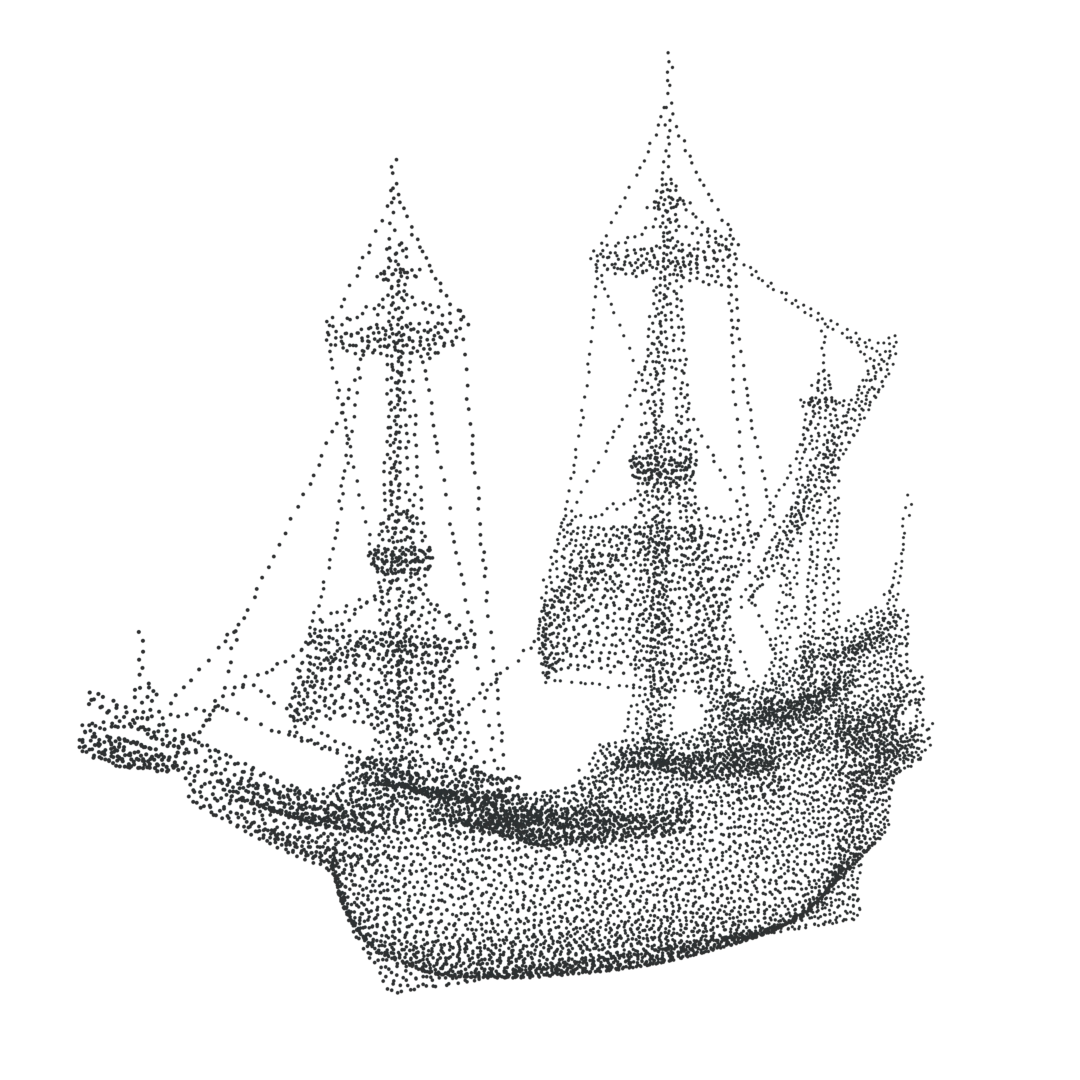
\includegraphics[width=\textwidth]{images/ship_sample_inv.png}
        \caption{Sampling of the mesh}
        \label{fig:ship-sample-b}
      \end{subfigure}\vspace{1cm}



      \begin{subfigure}[t][0.4\textwidth]{0.4\textwidth}
        \includegraphics[width=\textwidth]{images/ship_close.png}
        \caption{Close-up view of sails and ropes}
        \label{fig:ship-sample-c}
      \end{subfigure}
      \hfill
      \begin{subfigure}[t][0.4\textwidth]{0.4\textwidth}
        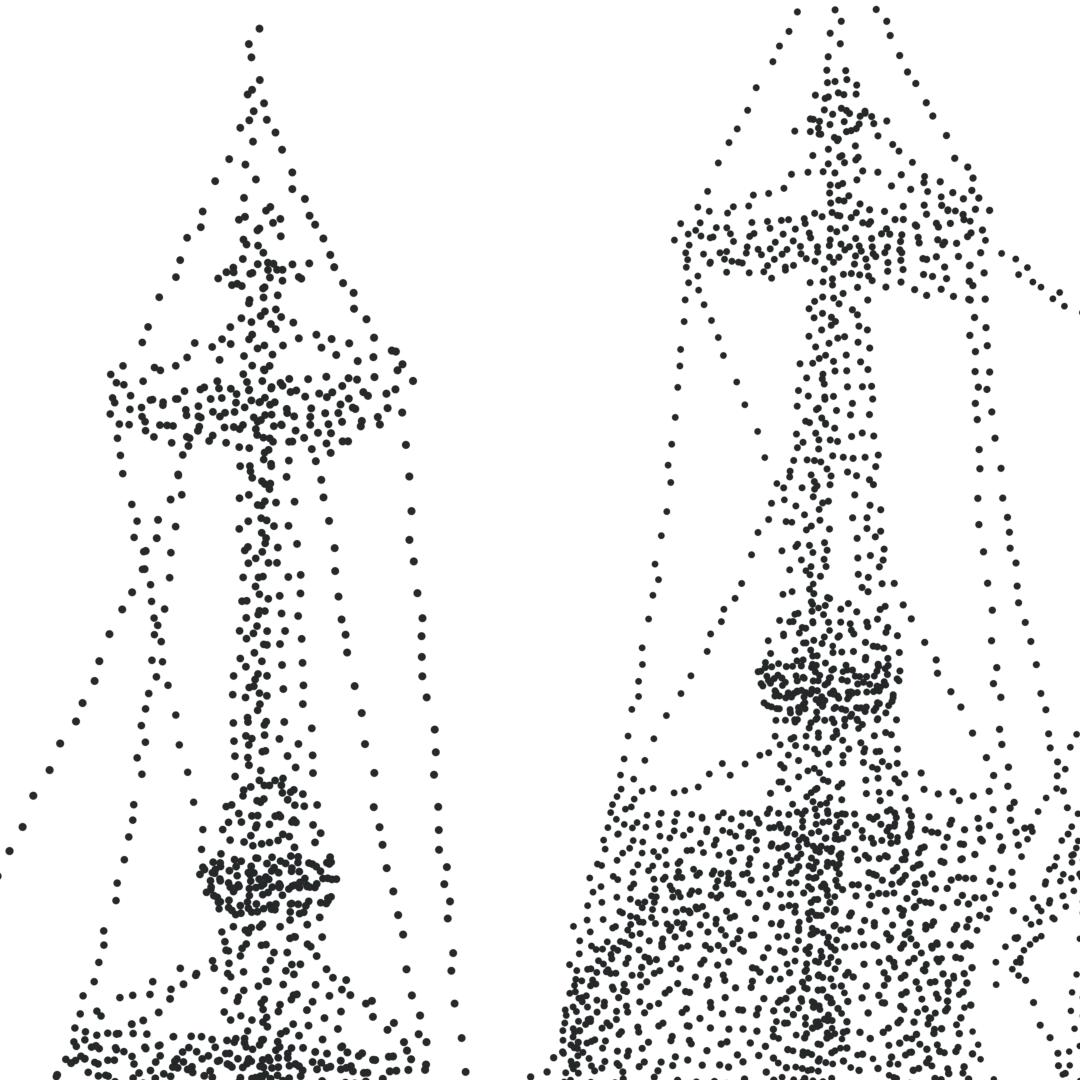
\includegraphics[width=\textwidth]{images/ship_sample_close_inv.png}
        \caption{Close-up view of sampled sails and ropes}
        \label{fig:ship-sample-d}
      \end{subfigure}
      \vspace{0.5cm}
      \caption{A rendering of a triangular mesh of a ship is shown in \autoref{fig:ship-sample-a}, with a close-up view of ropes and sails that are particularly challenging to sample in \autoref{fig:ship-sample-c}. The corresponding, low-discrepancy or blue noise samplings of boundary particles obtained by Poisson Disk sampling \autocite{pcu} are shown in \autoref{fig:ship-sample-b} and \autoref{fig:ship-sample-d} respectively, where particle positions are represented by small spheres. This highlights that the algorithm samples the mesh robustly even for complex and problematic geometries such as long, acute triangles in the ropes or non-manifold input geometry, at a resolution independent of that of the input mesh.}
      \label{fig:boundary-sampling}
    \end{figure}

    Both the Poisson disk sampling and resampling of the mesh as a watertight manifold are implemented in the \textit{Point Cloud Utils} library that was employed in the implementation discussed in this report \autocite{pcu}.

    \subsubsection{Boundary Particle Effective Mass}
    With the boundary particles' positions sampled on the boundary surface according to a blue noise distribution, a method for determining the effective mass of each boundary particle as it exerts forces upon a fluid particle is required to integrate the boundary formulation into the SPH sums in \autoref{sec:sph-navier-stokes}. As seen in \autoref{chp:sph}, the SPH sum approximates an integral over field quantities, which can be partitioned into an integral over the fluid domain $\Omega_{fl}$ and the boundary $\Omega_{bdy}$, which for the purpose of handling contact forces as pressure forces using the fluid solver can be assumed to be of the rest density $\rho_0$ of the fluid under consideration. Note that in this instance $\rho_0$ is fixed, for multiphase flows it can have differing values and in any case it is distinct from the actual mass density of the material, such as wood, stone or steel, being modelled by the boundary $\Omega_{bdy}$, which instead might influence the rigid body kinematics described in \autoref{sec:rigid-bodies}.

    For the density of a fluid particle near the boundary, one can write \autocite{density-maps}:
    \begin{align}
      \rho_i &= \int_{\Omega_{fl}} W_{ij} \,dm_j+  \int_{\Omega_{bdy}} W_{ik} \,dm_j\\
      \angled{\rho_i} &= \sum_{j\in\mathcal{N}_i} m_jW_{ij} + \sum_{k\in\mathcal{B}_i} m_k W_{ik}
    \end{align}
    where $\mathcal{B}$ is defined analogously to $\mathcal{N}$ but for boundary samples that neighbour particle $i$ and $m_k$ is the effective mass of a boundary particle assuming a boundary of density $\rho_0$ in $\Omega_{bdy}$.

    Since the entire boundary volume is represented by only a single layer of particles at the interface to the fluid, missing contributions and the variation in effective mass due to the non-uniform sampling must be accounted for. It is apparent that accurate values of $m_k$ would have to be at least a function of the distance to the interface in order to capture the fact that there are more missing boundary contributions in the kernel support of some fluid particle $i$ if it is close to the boundary. This could be approximated by linearly extending the boundary density field via $m_k = \rho_0 - \frac{\rho_0\cdot \abs{\vek{x}_{ik}}}{\hbar}$ using for example signed distance fields, storing the results on a grid and interpolating them as proposed by \autocite[Koshier and Bender]{density-maps}. Instead, for the small kernel support radius $\hbar=2h$ in the expected fluid particle spacing $h$, a constant approximation that is not distance-dependent can be deemed sufficiently accurate and more efficient, yielding the method of \autocite[Akinci et al.]{versatile-boundary-akinci}.

    With this piece-wise constant model, the effective mass that achieves a boundary domain with density $\rho_0$ is $m_k = \rho_0V_k$ where $V_k$ is the effective volume of the boundary domain represented by particle $k$. This in turn can be computed using the SPH normalization criterion \autoref{eq:normalization-0th-order} implying that $\sum_{l\in\mathcal{B}_k} V_l W_{kl}\overset{!}{=} 1$ ought to hold at any boundary particle $k$ \autocite{versatile-boundary-akinci}. This means that the kernel sum effectively measures the inverse of the volume of a particle given a sampling: if not $1$ but a higher value is obtained, all $V_l$ ought to be correspondingly lower and vice versa, which means \autocite{versatile-boundary-akinci}: 
    \begin{align}
      V_k = \frac{m_k}{\rho_0} &\overset{!}{=} \frac{m_k}{\sum_{l\in\mathcal{B}_k} m_l W_{kl}} \approx \gamma_1 \frac{ m_k}{m_k \sum_{l\in\mathcal{B}_k} W_{kl}}\label{eq:boundary-mass-approximation}\\
      \Longrightarrow m_k &= \gamma_1 \frac{\rho_0}{\sum_{l\in\mathcal{B}_k} W_{kl}}\label{eq:boundary-mass-calculation}
    \end{align}
    where the parameter $\gamma_1$ in the approximation can be used to adjust the density contribution per boundary particle for differing kernel support sizes, choosing for example a value that ensures rest density for a regular sampling of a plane, however $\gamma_1=1$ is chosen in this instance. 
    Since the effective mass is assumed to be independent of distance to the boundary, $m_k$ can be precomputed once and stored for each boundary particle.
    
    Instead of using the approximation of assuming roughly equal boundary masses in \autoref{eq:boundary-mass-approximation}, the exact equation can be seen as a system of equations and solved for $m_k$ in the same fashion as discussed for initializing fluid particles with rest density in \autoref{eq:initializing-fluid-rest-density}:
    \begin{align}
      m_k^0 &= \frac{\rho_0}{\sum_{l\in\mathcal{B}_k} W_{kl}}\\
      m_k^{l+1} &\gets m_k^l \cdot \frac{\rho_0}{\sum_{l\in\mathcal{B}_k} W_{kl}}\label{eq:boundary-mass-calculation-iterative}
    \end{align}

    In the implementation, the exact system is solved once initially, using \autoref{eq:boundary-mass-calculation-iterative}, since the one-off cost of the iterative solver is acceptable, but subsequent recalculations of masses due to dynamic boundaries are handled with a single application of the approximate formula \autoref{eq:boundary-mass-calculation} by \autocite[Akinci et al.]{versatile-boundary-akinci} to avoid additional runtime cost.
    
    \subsection{Dynamic and Procedural Boundaries}
    Not all boundaries are static: fluids might also interact with boundary particles representing dynamic rigid bodies simulated as described in \autoref{sec:rigid-bodies} or scripted boundaries, which behave according to some analytically specified equation of motion. In this implementation, scripted boundaries that implement rigid body translations were included, while rotations where neglected, since this limitation greatly simplifies the setting: given two equations $\vek{x}_{cm}(t), \vek{v}_{cm}(t)$, all boundary particles belonging to the same scripted object are shifted from their initial position by exactly $\vek{x}_{cm}(t)$ and all have the same velocity $\vek{v}_{cm}(t)$ at any point $t$ in time. 

    The previously discussed boundary handling can thankfully naturally handle intersecting boundaries. For example, a scripted boundary plane moving sinusoidally to produce waves may intersect a container of water. However, the masses of involved boundary particles might need to be recalculated so that the pressure forces exerted on the fluid by the boundary does not change where boundaries intersect. This is done according to two rules, which in conjunction conservatively estimate the set of boundary particles that need their masses recalculated according to \autoref{eq:boundary-mass-calculation} in each time step:
    \begin{enumerate}
      \item All masses of boundary particles belonging to scripted boundary objects are recalculated at every step. While performing the SPH kernel sum in \autoref{eq:boundary-mass-calculation} necessary to do so, all neighbouring particles $l$ have a counter set to 2 if they are static boundary samples.
      \item All static boundary samples with such a counter value greater than zero have their masses recalculated and the counter decremented.
    \end{enumerate}
    This means that not only are the masses of static boundary samples re-evaluated when scripted boundaries intersect them to ensure all boundary particles correctly exert forces on fluids as if they were the same fluid at rest density at all times, but the masses are also re-evaluated once more when a scripted boundary particle has just left the kernel support radius, ensuring correct masses as before. 
    
    Note that in the Taichi language used for this implementation, a quantized data type can be used to represent the counter since only 3 bits per boundary particle are required, which can be densely packed to reduce memory usage and possibly improve performance, see \autocite[Hu et al.]{quantized-taichi}

    \subsubsection{Extending the Governing Equations}\label{subsub:bdy-extend-governing}
    With the surfaces of boundary domains sampled using a blue-noise distribution and the effective boundary particle masses $m_k$ calculated such that they can be treated by the pressure solver like a fluid at rest with density $\rho_0$, the SPH discretized governing equations from \autoref{sec:sph-navier-stokes} can be extended to include the boundary domain.


    The density computation in \autoref{eq:discrete-density} is straightforward:
    \begin{equation}\label{eq:discrete-density-boundary}
      \angled{\rho_i} = \sum_{j\in\mathcal{N}_i} m_j W_{ij} + \sum_{k\in\mathcal{B}_i} m_k W_{ik}
    \end{equation}
    The viscosity computation in \autoref{eq:discrete-viscous} remains the same as before. While viscous forces at the boundary can be implemented and the symmetric forces acting on boundary particles can be integrated into the rigid body solver (see \autocite[Akinci et al.]{versatile-boundary-akinci}), slip-conditions were chosen instead in this implementation, since rather inviscid flows at larger scales are investigated.

    Lastly, the pressure computation must be adjusted. \autoref{eq:discrete-pressure} requires a density and pressure value per boundary particle $k$, which are unknown. Since the effective mass $m_k$ was chosen to represent $\rho_0$ in the boundary domain, the rest density $\rho_k\approx\rho_0$ is a reasonable approximation. For choosing a pressure value of a boundary particle, there exist many methods, such as simply mirroring the pressure of the fluid particle under consideration $p_i=p_k$ \autocite{versatile-boundary-akinci}, solving for pressures at boundary particles in the pressure solver explicitly to avoid inconsistent values of $p_k$ for different fluid particles $i$ \autocite{pressure-boundaries}{}, extrapolating the pressure field into the boundary domain using some scheme like \textit{Moving Least Squares} \autocite{mls-pressure-extrapolation}, or simply setting the pressure at boundary particles to zero \autocite{consistent-boundaries}. This choice can have a profound impact on pressure solver convergence and the quality of the resulting pressure field \autocite{consistent-boundaries}. In accordance with recent literature by \autocite[Bender et al.]{consistent-boundaries}, a so-called consistent boundary handling which imposes $p_k=0$ is chosen in this instance, which is exceptionally easy to implement, was found to improve solver stability and yield a reasonably smooth pressure field. It is equivalent to the approach of mirroring pressure values with a weighting of boundary pressure forces by a coefficient $\gamma_2=0.5$ \autocite{tutorial2019}. Using $p_k=0$, some terms in \autoref{eq:discrete-pressure} drop out, leaving the expression:
    \begin{equation}\label{eq:discrete-pressure-bdy}
      \vek{a}_i^p = \angled{-\frac{1}{\rho_i}\nabla p_i}_\parallel 
      = -\sum_{j\in\mathcal{N}_i} m_j \br{\frac{p_i}{\rho_i^2} + \frac{p_j}{\rho_j^2}} \nabla W_{ij} -\sum_{k\in\mathcal{B}_i} m_k\frac{p_i}{\rho_i^2} \nabla W_{ik}
    \end{equation}
    This expression is used to derive the diagonal element in the IISPH solver of \autoref{sec:iisph} using the additional assertion that $\rho_i\overset{!}{=}\rho_j\overset{!}{=}\rho_0$. Since this discretization of $\vek{a}_i^p$ makes use of the symmetric SPH approximation $\angled{\cdot}_\parallel$, one can easily derive the symmetric forces that the fluid particle $i$ exerts on each boundary particle $k$ using Newton's second law as \autocite{versatile-boundary-akinci}:
    \begin{equation}\label{force-on-bdy}
      f_{k\leftarrow i} = - m_i \vek{a}_{i\leftarrow k}^p = m_i m_k\frac{p_i}{\rho_i^2} \nabla W_{ik}
    \end{equation}
    which is used to exert forces and torques upon dynamic rigid bodies in \autoref{sec:rigid-bodies}.


    \section{Two-Way Coupled Rigid Body Solver}\label{sec:rigid-bodies}
    Assuming the mass properties of rigid bodies outlined in \autoref{sec:mass-moments} are known, the dynamics of unconstrained rigid bodies can be discussed in order to arrive at a solver which can be weakly coupled to the fluid solver from \autoref{chp:fluid}. Two-way coupling is achieved through two interfaces between the fluid and rigid solvers:
    \begin{enumerate}
      \item By sampling the boundary of the rigid body as explained in \autoref{sec:boundary} and moving the boundary particles as the rigid body moves, contact with the fluid is resolved in the same way as for static boundaries which exhibit one-way coupling: pressure forces computed by the fluid solver in \autoref{sec:iisph} resolve penetrations and keep the fluid from leaking into the rigid body.
      \item On the other hand, the fluid must also exert forces and torques on the rigid body, influencing its movement and creating two-way coupling. This was alluded to in \autoref{force-on-bdy}, where the pressure force exerted on a boundary particle by a fluid particle was formulated.
    \end{enumerate}

    These interfaces define the inputs and outputs of the rigid body solver. It takes a state of a rigid body and all the forces and torques that act on it, then computes an updated state of the body and finally moves all particles that sample the rigid body boundary to reflect the changes in the rigid body's state.
    These three steps are outlined in the following.

    \subsubsection{Forces and Torques}
    As per Chasles' theorem, rigid body motion can be described purely by the position and rotation of the body \autocite{classical-mechanics}, since ideal rigidity means that the relative positions of each two points in the body do not change and no other deformations such as observed in elastic bodies or fluids can occur. This means that the dynamics can be split into the two separate problems of computing the linear and angular movement of the body \autocite{classical-mechanics}. This is conveniently done by using the centre of mass $\vek{x}_{cm}$ as the origin which defines \textit{body space}. In this coordinate system, any point $\vek{x}'(t) := \vek{x}(t) - \vek{x}_{cm} $ belonging to the rigid body can be described using the equation of motion \autocite{physically-based-rigids}:
    \begin{equation}\label{eq:rigid-body-equation-of-motion}
      \vek{x}(t) = \mathds{O}(t)\vek{x}'(t=0) + \vek{x}_{cm}(t)
    \end{equation}
    where $\mathds{O}$ encodes the current rotation about the centre of mass in a rotation matrix and $\vek{x}_{cm}(t)$ is the position of the centre of mass in world space. This means that all rotational aspects of the motion are encoded in the orientation $\mathds{O}$, while the translational movement only affects the position and velocity of the centre of mass. 
    
    Accordingly, for the change in linear momentum $\vek{f}_{rigid} = \frac{d}{dt} M\vek{v}_{cm}$ and constant mass $M$ it holds that all forces $\vek{f}_i$ affecting the rigid body (in this instance the symmetric pressure forces in \autoref{force-on-bdy}) can simply be summed, including the external gravitational force acting on the body \autocite{physically-based-rigids}:
    \begin{equation}\label{eq:f-rigid}
      \vek{f}_{rigid} = \vek{f}_g + \sum_i \vek{f}_i
    \end{equation}
    irrespective of the position at which each force acts on the rigid body. This results in a single net translational force, which can be interpreted as an acceleration $\vek{a}_{cm} = \frac{1}{M}\vek{f}_{rigid}$ of the centre of mass $\vek{x}_{cm}$ and integrated with respect to time as in \autoref{eq:numerical-time-integration}.

    Meanwhile, the rate of change of the angular momentum  $\frac{d}{dt}\vek{L}=\vek{\tau}_{rigid}$ defines the net torque $\vek{\tau}_{rigid}$, which can be computed as \autocite{physically-based-rigids}:
    \begin{equation}\label{eq:rigid-net-torque}
      \vek{\tau}_{rigid} = \sum_i \vek{\tau}_i = \sum_i (\vek{x}_i-\vek{x}_{cm}) \times \vek{f}_i
    \end{equation}
    where the position $\vek{x}_i$ in world space at which the force $\vek{f}_i$ acts upon the rigid body is relevant. Intuitively, the vector $\vek{\tau}_i$ can be understood as pointing in the axis of the rotation that a force $\vek{f}_i$ would cause if the rigid body was fixed at its centre of mass and left to spin \autocite{physically-based-rigids}.
    
    \subsubsection{Updating Rigid Body State}
    Using the total input force $\vek{f}_{rigid}$ and torque $\vek{\tau}_{rigid}$, the state of the rigid body at the next time step $t+\Delta t$ must be computed from its current state. To obtain the updated position of the centre of mass $\vek{x}_{cm}\br{t+\Delta t}$ and the orientation $\mathds{O}\br{t+\Delta t}$ required to solve the equation of motion (\autoref{eq:rigid-body-equation-of-motion}), the corresponding differential quantities, namely the linear velocity $\vek{v}_{cm}$ and angular velocity $\vek{\omega}$ are required and are integrated with respect to time. 

    The linear velocity and updated centre of mass are straightforward and can be obtained using for example semi-implicit Euler time integration (\autoref{eq:numerical-time-integration}) from the linear acceleration described above as:
    \begin{align}
      \vek{v}_{cm}(t+\Delta t) &= \vek{v}_{cm}(t) + \Delta t \vek{a}_{cm}\br{t} = \vek{v}_{cm}(t) + \frac{\Delta t}{M} \vek{f}_{rigid}\br{t}\label{eq:rigid-vcm-update}\\
      \vek{x}_{cm}\br{t+\Delta t} &= \vek{x}_{cm}\br{t} + \Delta t \vek{v}_{cm}(t+\Delta t)\label{eq:rigid-xcm-update}
    \end{align}

    The angular velocity $\vek{\omega}$ points in the axis of rotation with a magnitude that encodes the speed of the revolution in radians per second \autocite{physically-based-rigids}. Analogous to how the linear velocity is related through mass to the linear momentum, the angular velocity is related through the inertia tensor to the angular momentum \autocite{classical-mechanics}:
    \begin{align}
      \vek{L}\br{t} &= \mathds{I}\br{t} \vek{\omega}\br{t}\\
      \mathds{I}\br{t}^{-1} \vek{L}\br{t} &=\vek{\omega}\br{t}\label{eq:rigid-update-omega-deriv}
    \end{align}
    where the angular momentum can be found by numerically integrating the torque with respect to time, since $\vek{\tau}=\frac{d}{dt}\vek{L}$ \autocite{physically-based-rigids}:
    \begin{equation}
      \vek{L}\br{t+\Delta t} = \vek{L}\br{t} + \Delta t \vek{\tau}_{rigid}\br{t}
    \end{equation}
    The inertia tensor (or its inverse) at some point in time $t$ can be determined as \autocite{physically-based-rigids}:
    \begin{align}
      \mathds{I}\br{t} &= \mathds{O}\br{t} \mathds{I}\br{t=0} \mathds{O}\br{t}^T\\
      \mathds{I}^{-1}\br{t} &= \mathds{O}\br{t} \mathds{I}^{-1}\br{t=0} \mathds{O}\br{t}^T
    \end{align}
    in terms of the initial inertia tensor $\mathds{I}\br{t=0}$ that is computed in \autoref{subsubsec:inertia-tensor-computation}. Note that since $\mathds{O}$ is a rotation matrix, the transpose of the matrix is its inverse. 

    The orientation $\mathds{O}$ can be updated using:
    \begin{equation}\label{eq:rigid-orientation-update}
      \mathds{O}\br{t+\Delta t} = \mathds{O}\br{t} + \Delta t \dot{\mathds{O}}\br{t}
    \end{equation}
    where $\dot{\mathds{O}}\br{t}$ or the rate of change of the orientation matrix is the skew-symmetrix matrix that encodes the angular velocity $\vek{\omega}\br{t} = \br{\omega_x, \omega_y, \omega_z}^T$, namely \autocite{physically-based-rigids}:
    \begin{equation}
      \dot{\mathds{O}}\br{t} = \begin{bmatrix}
        0&-\omega_z&\omega_y\\
        \omega_z&0&-\omega_x\\
        -\omega_y&\omega_x&0
      \end{bmatrix}
    \end{equation}
    With this, the orientation can be updated and the angular velocity at the next time step can be estimated using \autoref{eq:rigid-update-omega-deriv} as:
    \begin{align}\label{eq:rigid-update-omega}
      \vek{\omega}\br{t+\Delta t} &= \mathds{I}^{-1}\br{t+\Delta t} \vek{L}\br{t+\Delta t}\\
      &= \mathds{O}\br{t+\Delta t} \mathds{I}^{-1}\br{t=0} \mathds{O}\br{t+\Delta t}^T \vek{L}\br{t+\Delta t}
    \end{align}

    \subsubsection{Orthonormalization of $\mathds{O}$ and Quaternions}
    In \autoref{eq:rigid-orientation-update}, the orientation is updated by explicitly numerically integrating a differential change in orientation. Unfortunately, after this process, the orientation $\mathds{O}$ is not guaranteed to be a rotation matrix any more. Numerical drift can lead to accumulating errors, potentially leading to an unphysical scaling or skew of the rigid body \autocite{physically-based-rigids}, indicated by the determinant $\det\br{\mathds{O}}$ becoming different from one. To prevent this, $\mathds{O}$ could be re-orthonormalized after every so often, using for example the Gram-Schmidt process. However, this would cause the error to be projected onto arbitrarily chosen axes that depend on the order of the basis vectors considered in the process. A more elegant approach is choosing a different representation of orientations that can alleviate this issue.

    One such representation are quaternions, which extend the concept of complex numbers to four instead of two dimensions. A quaternion $s + x i + y j + z k$ has, in addition to the imaginary unit $i$, the basis vectors $j$ and $k$, and can be represented by a single vector $\vek{q} = \br{s,x,y,z}^T$ in four dimensions or a pair $\left[s,\vek{v}\right]$ of a scalar $s$ and a vector $\vek{v}=\br{x,y,z}^T$ holding its coefficients \autocite{physically-based-rigids}. Using the second definition, quaternion multiplication can be written as \autocite{physically-based-rigids}:
    \begin{align}
      \vek{q}_1 \vek{q}_2 
      &= \left[s_1,\vek{v}_1\right] \left[s_2,\vek{v}_2\right] \\
      &= \left[s_1 s_2 - \vek{v}_1 \cdot \vek{v_2}, s_1\vek{v}_2 + s_2\vek{v}_1 + \vek{v}_1 \times \vek{v}_2 \right]
    \end{align}
    which is not commutative. If a quaternion has unit length, it represents a rotation and the product of two such quaternions represents the composite of each rotation in sequence \autocite{physically-based-rigids}, making them especially convenient in this context. It turns out that the rate of change of the orientation $\dot{\vek{q}}$ can be expressed in terms of the angular velocity $\vek{\omega}$ using quaternion multiplication as:
    \begin{equation}\label{eq:rigid-quaternion-qdot}
      \dot{\vek{q}} = \frac{1}{2} \left[0,\vek{\omega}\right]\left[s,\vek{v}\right] 
    \end{equation}
   This can be explicitly numerically integrated:
    \begin{equation}\label{eq:rigid-qdot-integration}
      \vek{q}\br{t+\Delta t} = \vek{q}\br{t} + \Delta t\dot{\vek{q}}\br{t}
    \end{equation}
    and then normalized like any four-dimensional vector, so it remains a representation of a rotation. Finally, the resulting unit quaternion $\hat{\vek{q}}\br{t+\Delta t}=\br{s,x,y,z}^T$ can be converted to a rotation matrix $\mathds{O}\br{t+\Delta t}$  using the identity \autocite{physically-based-rigids}:
    \begin{equation}\label{eq:rigid-quaternion-to-matrix}
      \mathds{O} = \begin{bmatrix}
        1-2y^2-2z^2 & 2xy-2sz & 2xz+2sy\\
        2xy+2sz & 1-2x^2-2z^2 & 2yz-2sx\\
        2xz-2sy & 2yz+2sx & 1-2x^2-2y^2\\
      \end{bmatrix}
    \end{equation}
    which can be used as an auxiliary variable to compute $\mathds{I}^{-1}\br{t+\Delta t}$ and $\vek{\omega}\br{t+\Delta t}$ as outlined above, but does not need to be stored any more since $\vek{q}$ is now used to represent the current orientation of the rigid body. Note that the initial orientation can be encoded by $\hat{\vek{q}}\br{t=0} = \br{1,0,0,0}^T$.

    \subsubsection{Updating the Dynamic Boundary Particles}
    Once a new orientation $\mathds{O}\br{t+\Delta t}$ and position of the centre of mass $\vek{x}_{cm}\br{t+\Delta t}$ has been obtained, all boundary particles sampled on the surface of the rigid body can be moved according to \autocite{physically-based-rigids}:
    \begin{align}
      \vek{r}_i\br{t+\Delta t} &= \mathds{O}\br{t+\Delta t} \br{\vek{x}_i\br{t=0} - \vek{x}_{cm}\br{t=0}}\\
      \vek{x}_i\br{t+\Delta t} &= \vek{r}_i\br{t+\Delta t} + \vek{x}_{cm}\br{t+\Delta t}\label{eq:rigid-update-particle-x}\\
      \vek{v}_i\br{t+\Delta t} &= \vek{v}_{cm} + \vek{\omega}\br{t+\Delta t} \times \vek{r}_i\br{t+\Delta t}\label{eq:rigid-update-particle-v}
    \end{align}
    using the initial positions at $t=0$, where $\vek{r}_i$ was introduced for readability and need not be stored. 

    All the steps necessary to perform a single update of a rigid body are summarized in Algorithm \ref{alg:rigid-sim}.

    
    \begin{algorithm}
      \caption{Rigid Body Solver Step}
      \label{alg:rigid-sim}
      \begin{algorithmic}[1]
        \Phase{Compute Linear Movement}

        \State $\vek{v}_{cm} \gets \vek{v}_{cm} + \Delta t \br{\vek{g} + \frac{1}{M}\sum_i\vek{f}_i}$ \Comment{\autoref{eq:rigid-vcm-update}}
        \State $\vek{x}_{cm} \gets \vek{x}_{cm} + \Delta t \vek{v}_{cm}$ \Comment{\autoref{eq:rigid-xcm-update}}
        
        \Phase{Update Orientation}
        \State $\dot{\vek{q}} \gets \frac{1}{2} \left[0,\vek{\omega}\right]\vek{q}$ \Comment{\autoref{eq:rigid-quaternion-qdot} using quaternion multiplication}
        \State $\vek{q} \gets \frac{\vek{q} + \Delta t \dot{\vek{q}}}{\abs{\vek{q} + \Delta t \dot{\vek{q}}}}$ \Comment{\autoref{eq:rigid-qdot-integration} and normalize quaternion}
        \State Calculate $\mathds{O}$ from $\vek{q}$ \Comment{\autoref{eq:rigid-quaternion-to-matrix}}

        \Phase{Compute Rotational Movement}
        \State $\vek{L} \gets \vek{L} + \Delta t \vek{\tau}_{rigid}$ \Comment{using $\vek{\tau}_{rigid}$ from \autoref{eq:rigid-net-torque}}
        \State $\vek{\omega} \gets \mathds{O} \mathds{I}^{-1}\br{t=0} \mathds{O}^T \vek{L}$ \Comment{\autoref{eq:rigid-update-omega}}

        \Phase{Update Particles}
        \For{$i \in \mathds{N}_0^{N_{rigid}-1}$ in parallel}
          \State $\vek{r}_{i,0} = \br{\vek{x}_i\br{t=0} - \vek{x}_{cm}\br{t=0}}$ \Comment{Initial body space position, auxiliary variable}
          \State $\vek{x}_i \gets \mathds{O} \vek{r}_{i,0} + \vek{x}_{cm}$ \Comment{\autoref{eq:rigid-update-particle-x}}
          \State $\vek{v}_i \gets \vek{v}_{cm} + \vek{\omega}\times \br{\mathds{O}\vek{r}_{i,0}}$ \Comment{\autoref{eq:rigid-update-particle-v}}
        \EndFor
      \end{algorithmic}
    \end{algorithm}
    
    

    
  \subsection{Exact Mass Moments of Watertight Meshes}\label{sec:mass-moments}
  In order to implement the rigid body solver in \autoref{sec:rigid-bodies}, prerequisite include knowing the total mass $M$, centre of mass $\vek{x}_{cm}$, volume $V$ and the inertia tensor $\mathds{I}$ of the rigid body being simulated. As an input to this computation, some arbitrary triangular mesh is given, which can be approximated by a watertight manifold using the algorithm discussed in \autoref{subsec:sampling-the-boundary}, which is in turn interpreted as the surface $\partial\Omega_{rigid}$ of some volume $\Omega_{rigid}$ that represents a rigid body of homogeneous density $\rho$. In other words, the mass moments necessary for the computation of $M,\mathds{I},\vek{x}_{cm}$ etc. of the closed triangular mesh of $\partial\Omega_{rigid}$ must be computed, in this case using a method by \autocite[Zhang and Chen]{efficient-feature-extraction}, which is outlined in the following. The mass density moments of the $\Omega_{rigid}$ are defined as an integral \autocite{efficient-feature-extraction}:
  \begin{equation}\label{eq:mass-density-moments}
    \mathcal{M}_{pqr} := \iiint_{\Omega_{rigid}} \rho x^p y^q z^r  \, dxdydz
  \end{equation}
  over the volume of the rigid body for some $p,q,r$, which means that the zero-th moment $p=q=r=0$ is the total mass of the object, the first moment $p=q=r=1$ is used to calculate the centre of mass, and the entries of the inertia tensor can be computed from some other $p,q,r \in \mathds{N}_0^2$ that are discussed in \autoref{subsubsec:inertia-tensor-computation}.

  \subsubsection{Volume Integrals as Sums over Triangles}
  
  Using the fact that the input triangular mesh is now a closed manifold, there exists a method for computing the analytic mass moment of the mesh. 
  
  The method makes use of the notion of signed volumes $V'$ of tetrahedra, where given some vertex $O$ of a tetrahedron and the triangle $\triangle_{ABC}$ formed by its remaining, ordered vertices, it is assigned either a positive or a negative volume depending on whether the normal of the triangle $\triangle_{ABC}$ faces towards or away from $O$. Note that since the input mesh is now a watertight manifold, each connected component of the mesh defines an interior and an exterior, consists of triangles and can be stored in a consistent winding order such that the normals $\frac{\overrightarrow{AB} \times \overrightarrow{AC}}{\abs{\overrightarrow{AB} \times \overrightarrow{AC}}}$ all point towards the exterior, as is convention, or all point towards the interior. In this instance, counter-clockwise winding was used, but differing input meshes can be accounted for by flipping the sign of the signed volume accordingly.
  
  More traditionally, the integration domain $\Omega_{rigid}$ could be partitioned into a set of tetrahedra $\{\tetrahedron_i\}$ such that $\Omega_{rigid} = \bigcup_i \tetrahedron_i$ and $\forall i,j: \tetrahedron_i \cap \tetrahedron_j = \emptyset$ so that the integral can be written as:
  \begin{equation}
    \int_{\Omega_{rigid}} \,dV = \sum_{\tetrahedron_i} V\br{\tetrahedron_i}
  \end{equation} where $V\br{\tetrahedron_i}$ is the volume of the $i$-th tetrahedron that can be computed analytically from its vertices. This would necessitate a decomposition into tetrahedra that is neither trivial nor efficient. 
  
  Instead, one fixed point $O$ anywhere in space can be chosen to construct tetrahedra $\tetrahedron_{ABCO}$ by simply summing over all the triangles $\triangle_{ABC}$ in the mesh and appending the vertex $O$ to form a tetrahedron. These tetrahedra no longer partition space, so a simple sum over their volumes would not yield the correct total volume of the domain but some possibly larger value. However, the crucial insight lies in the fact that summing up the signed volumes $V'\br{\tetrahedron_{ABCO}}$ with a consistent winding order as described above results in multiply accounted for volumes outside $\Omega_{rigid}$ exactly cancelling out, leaving only the volume inside $\Omega_{rigid}$, which is accounted for an odd number of times with alternating signs. This is conceptually simlar to how parity of the number of intersections along a ray is used to determine if a point lies inside a polygon as per the Jordan Curve theorem in \autoref{subsec:initial-conditions}, only the parity of faces with normals oriented towards or away from some vertex $O$ is now used to determine subvolumes inside or outside the mesh. \autoref{fig:volume-integral-triangle-mesh} might make this concept clearer by illustrating a concrete example in two dimensions. 
  
  %The intuition here is similar to the Jordan Curve theorem mentioned in \autoref{subsec:initial-conditions}: if a ray from an $O$ outside of the mesh to some point on $\triangle_{ABC}$ is imagined, then just as the number of intersections of the ray with $\partial\Omega_{rigid}$ indicates whether a point along the ray is inside or outside the domain depending on if the number of intersections is even or odd, the ray also alternates between intersecting faces with normals in or against the ray direction, and in consequence the volume containing some point on the ray is described by an even number of terms in the sum of signed volumes with alternating signs that therefore cancel to zero, or an odd number that is always negative or always positive. \autoref{fig:volume-integral-triangle-mesh} makes this much clearer by showing a concrete example in two dimensions. 

  \begin{figure}
    \begin{center}
      \begin{asy}
import geometry;
import patterns;
size(10cm);
pair[] P = {(-1,2),(2,2.5),(5,4),(4,1)};
pair[] directions = {W, NW, NE, SE};
pair O = (1,0);

pen hatchpen = black+opacity(0.8)+linewidth(0.1);
add("hatch1",hatch(H=1.1mm, dir=NE, p=hatchpen));
add("hatch2",hatch(H=1.1mm, dir=NW, p=hatchpen));

pen style1 = red+opacity(0.2);
pen style2 = blue+opacity(0.2);
pen poly_pen = linewidth(1.0) + black;

path poly = P[0];
for (int i = 0; i < P.length; ++i) {
pair dir = directions[i % directions.length];
dot(P[i]);
label("$V_"+string(i)+"$", P[i], dir);
poly = poly -- P[i];
}
poly = poly -- cycle;
draw(poly, poly_pen);

dot(O); label("$O$", O, S);

bool isNormalTowardsO(pair A, pair B, pair O) {
pair AB = B - A;
pair AO = O - A;
real cross = AB.x * AO.y - AB.y * AO.x;
return cross > 0;
}

for (int i = 0; i < P.length; ++i) {
pair A = P[i];
pair B = P[(i+1) % P.length]; 
if (isNormalTowardsO(A, B, O)) {
  filldraw(A -- B -- O -- cycle, style1);
} else {
  filldraw(A -- B -- O -- cycle, style2);
}
}
for (int i = 0; i < P.length; ++i) {
pair A = P[i];
pair B = P[(i+1) % P.length];
if (isNormalTowardsO(A, B, O)) {
  fill(A -- B -- O -- cycle, pattern("hatch1"));
} else {
  fill(A -- B -- O -- cycle, pattern("hatch2"));
}
}
        \end{asy}
        \caption{In a figure similar to the one by \autocite[Zhang and Chen]{efficient-feature-extraction}, a volume integral using the described method of signed volumes is illustrated for a polygon with vertices $V_0,V_1,V_2,V_3$ and an additional vertex $O$ at the origin. Whereas in three dimensions, volumes of tetrahedra are added, and we sum over the triangles of a mesh, in this two-dimensional setting the areas of triangles are added in a sum over edges of the mesh. Positive signed areas are coloured blue and hatched along one diagonal, negative areas are red and hatched along the other diagonal. The purple, cross-hatched area outside the mesh is therefore added once and subtracted once, resulting in a net contribution to the total area of zero, while the area inside the polygon does not cancel out and remains as the result of the computation.}
        \label{fig:volume-integral-triangle-mesh}
      \end{center}
  \end{figure}

  Since the fixed point $O$ is arbitrary, the most computationally efficient choice is $O=\br{0,0,0}^T$. With this choice, the signed volume of any tetrahedron $\tetrahedron_{ABCO}$ can be defined as \autocites{efficient-feature-extraction}{explicit-exact-tetrahedron-formulas}:
  \begin{align}
    V'\br{\tetrahedron_{ABCO}} &= \frac{1}{6}\det\br{J\br{\tetrahedron_{ABCO}}}\\
    &= \frac{1}{6}\det\br{\begin{bmatrix}
    A_x&B_x&C_x\\A_y&B_y&C_y\\A_z&B_z&C_z
    \end{bmatrix}}\\
    &= \frac{1}{6}\br{\vek{A} \times \vek{B}} \cdot \vek{C}\label{eq:tetrahedron-signed-volume-determinant}
  \end{align}
  where $J$ denotes the Jacobian of the tetrahedron and the position vector of each vertex $\overrightarrow{OA}=\vek{A}$ etc. can be used in the Jacobian since $O$ was chosen to be the origin. The triple scalar product used to compute the determinant is anticommutative, so the order of any two of the vectors $\vek{A},\vek{B},\vek{C}$ in the expression above can be swapped to alternate the sign of the result, for example to account for a different winding order. With this, the volume integral can be written as a sum \autocite{efficient-feature-extraction}:
  \begin{equation}\label{eq:tetrahedron-signed-volume-sum}
    V\br{\Omega_{rigid}} = \int_{\Omega_{rigid}} \,dV = \abs{\sum_{\triangle_{ABC}} V'\br{\tetrahedron_{ABCO}}}
  \end{equation}
  From now on, it will be assumed that the winding order and the order of the vectors in \autoref{eq:tetrahedron-signed-volume-determinant} were chosen such that the sum of signed volumes are always positive and the absolute value $\abs{\cdot}$ in \autoref{eq:tetrahedron-signed-volume-sum} could be dropped. In other words, $\sum_{\triangle_{ABC}} V'\br{\tetrahedron_{ABCO}}$ being a positive quantity defines some function $\sgn\br{\tetrahedron_{ABCO}}\in\{-1,1\}$, which assigns a positive or negative weight to any tetrahedron $\tetrahedron_{ABCO}$, yielding the sign of its signed volume $V'$.

  One of the greatest properties of this method, apart from its exact accuracy for closed meshes, is that it generalizes to any mass moments as defined in \autoref{eq:mass-density-moments} through the relation \autocite{efficient-feature-extraction}:
  \begin{equation}\label{eq:mass-density-moments-using-signed-volume}
    \mathcal{M}_{pqr} = \sum_{\triangle_{ABC}} \br{\sgn\br{\tetrahedron_{ABCO}} \cdot \iiint_{\Omega\br{ABCO}} \rho x^p y^q z^r  \,dV}
  \end{equation}
  where $\Omega\br{ABCO}$ is the domain of the tetrahedron $\tetrahedron_{ABCO}$, for which exact analytic solutions to the triple integral exist when homogeneous density is assumed, as outlined in \autoref{chp:analytic-tetrahedron-inertia}.
  % Instead of integrating a quantity over a volume inside a triangular mesh by, for example, partitioning it into tetrahedra and summing up the analytic expressions for the integral over each tetrahedron, one additional fixed point $O$ anywhere in space can be used to construct a sum over tetrahedra $OABC$ for each triangle $ABC$ in the triangular mesh. 
  
  
  % Whereas a volume integral $\int_{\Omega_{rigid}} \,dV$ can be written as the sum of volumes of tetrahedra $\sum_{ABCD} V_{ABCD}$ for each tetrahedron $ABCD$ that partitions $\Omega_{rigid}$, the integral can now also be written as the sum of signed volumes $\sum_{ABC} V_{ABCO}'$, which is simply a sum over the triangles $ABC$ in the triangular mesh and does not require a possibly expensive decomposition into tetrahedra. 
  
  % The crucial insight into why this method works is similar to the Jordan curve theorem, except the intuition is lifted from rays to volumes as per the Jordan any volume inside the rigid body domain is accounted for an odd number of times, volumes outside are accounted for an even number of times and the sign of the signed volume alternates at every intersection with the surface $\partial\Omega_{rigid}$.
  
  \subsubsection{Zeroth Mass Density Moment: Total Mass}
  It follows that the total mass of a rigid body of homogeneous density $\rho$ is:
  \begin{equation}\label{eq:total-rigid-body-mass}
    M\br{\Omega_{rigid}} = \int_{\Omega_{rigid}} \rho \,dV= \mathcal{M}_{000}  = \sum_{\triangle_{ABC}} V'\br{\tetrahedron_{ABCO}} \rho  =:  \sum_{\triangle_{ABC}} M'\br{\tetrahedron_{ABCO}}
  \end{equation}
  which can be efficiently and conveniently computed for each face of the mesh in parallel and summed up using a parallel reduction.

  \subsubsection{First Mass Density Moments: Centre of Mass}\label{subsubsec:centre-of-mass}
  Describing changes of linear momentum of a rigid body is conveniently done by applying forces to the centre of mass, which is defined as:
  \begin{equation}
    \vek{x}_{cm}\br{\Omega_{rigid}} = \frac{1}{M\br{\Omega_{rigid}}}\int_{\Omega_{rigid}} \vek{x}' \cdot \rho\br{\vek{x}'} \, dV\br{\vek{x}'} = \frac{1}{\mathcal{M}_{000}}\begin{bmatrix}
      \mathcal{M}_{100}\\
      \mathcal{M}_{010}\\
      \mathcal{M}_{001}
    \end{bmatrix}
  \end{equation}
  Since the centre of mass of any tetrahedron is its centroid, the signed centre of mass of each tetrahedron in the sum can be given in terms of the signed mass $M'\br{\tetrahedron_{ABCO}}$ from \autoref{eq:total-rigid-body-mass}:
  \begin{equation}
    \vek{x}_{cm}\br{\tetrahedron_{ABCO}} = \frac{M'\br{\tetrahedron_{ABCO}}}{4}\br{\vek{A}+\vek{B}+\vek{C}}
  \end{equation}
  which means the centre of mass of the entire rigid body can be computed as:
  \begin{equation}
    \vek{x}_{cm} = \frac{1}{M} \sum_{\triangle_{ABC}}\vek{x}_{cm}\br{\tetrahedron_{ABCO}}
  \end{equation}

  \subsubsection{Second Mass Density Moments: Inertia Tensor}\label{subsubsec:inertia-tensor-computation}
  To describe how torques create rotations of rigid bodies, the inertia of the body about any axis has to be known. The inertia can be thought of as the quotient of the angular momentum $\vek{L}$ and the angular velocity $\vek{\omega}$, yielding a second rank tensor $\mathds{I}$ which is a $3\times 3$ matrix in three dimensions with diagonal elements called \textit{moments of inertia} and non-diagonals referred to as \textit{products of inertia} \autocite{classical-mechanics}. The eigenvectors of the inertia tensor are the principal axes of rotation; it is a symmetric tensor with six degrees of freedom and is defined as \autocites{fast-accurate-polyhedral-mass-properties}{classical-mechanics}:
  \begin{equation}\label{eq:inertia-tensor-long-definition}
    \mathds{I} = \begin{bmatrix}
      \int_\Omega \rho\br{x,y,z} \br{y^2+z^2} \,dV&
      -\int_\Omega  \rho\br{x,y,z} xy \,dV&
      -\int_\Omega  \rho\br{x,y,z} xz \,dV\\
      -\int_\Omega  \rho\br{x,y,z} yx \,dV&
      \int_\Omega  \rho\br{x,y,z} \br{x^2+z^2} \,dV&
      -\int_\Omega  \rho\br{x,y,z} yz \,dV\\
      -\int_\Omega  \rho\br{x,y,z} zx \,dV&
      -\int_\Omega  \rho\br{x,y,z} zy \,dV&
      \int_\Omega   \rho\br{x,y,z} \br{x^2+y^2} \,dV\\
    \end{bmatrix}
  \end{equation}
  Note that the symmetry $I_{ab} = I_{ba}$ results in the six degrees of freedom and that for homogeneous density, $\rho$ can be moved out of the integral. Further, since $\int_\Omega x^2+y^2\,dV = \int_\Omega x^2\,dV + \int_\Omega y^2\,dV$, the inertia tensor can be written in terms of the mass density moments $\mathcal{M}_{pqr}$ as:
  \begin{align}
    \mathds{I} &= \begin{bmatrix}
      I_{xx}&-I_{xy}&-I_{xz}\\
      -I_{xy}&I_{yy}&-I_{yz}\\
      -I_{xz}&-I_{yz}&I_{zz}
    \end{bmatrix}\\
    I_{xx} &= \mathcal{M}_{200}\\
    I_{yy} &= \mathcal{M}_{020}\\
    I_{zz} &= \mathcal{M}_{002}\\
    I_{xy} &= \mathcal{M}_{100} + \mathcal{M}_{010}\\
    I_{xz} &= \mathcal{M}_{100} + \mathcal{M}_{001}\\
    I_{yz} &= \mathcal{M}_{010} + \mathcal{M}_{001}
  \end{align}
  where \autoref{eq:mass-density-moments-using-signed-volume} can be applied to calculate each invocation of $\mathcal{M}$ efficiently. In \autoref{eq:mass-density-moments-using-signed-volume}, the analytic solution to volume integrals over tetrahedra $\tetrahedron_{ABCO}$ are required, which in this instance have the form:
  \begin{align}
    \rho \int_{\Omega\br{ABCO}} x^2+y^2\, dV\\
    \rho \int_{\Omega\br{ABCO}} xy\, dV
  \end{align}
  and analogously for the other two axes. These exact analytic expressions are cited from \autocite[Tonon]{explicit-exact-tetrahedron-formulas} and moved to \autoref{chp:analytic-tetrahedron-inertia} since they are rather verbose. Using \autoref{eq:inertia-appendix-final-eq}, the final inertia tensor $\mathds{I}$ can be computed. With this, all quantities are known and a simple rigid body solver as discussed in \autoref{sec:rigid-bodies} can be implemented.


\chapter{Visualization}\label{chp:visualization}
    \section{Spray, Foam and Bubble Generation}
    \section{Rendering}
\chapter{Analysis}\label{chp:analysis}
    \section{Solver Convergence}
    \section{Source Terms and Stability}
    \section{Performance Scaling}

\begin{appendices}
    \chapter{Fixed Radius Neighbour Search}
    There exist numerous methods for implementing the computation of the neighbour sets $\mathcal{N}_i = \{j : \abs{\vek{x}_{ij}}<\hbar\}$ referred to in \autoref{sec:sph-discretization}. In this implementation, a GPU-friendly index sort based on counting sort was implemented as an implicit representation of a uniform grid to speed up neighbour computation, following the description of \autocite[Hoetzlein]{hoetzlein-rama-counting-sort}. 

    It is apparent that a na\"ive neighbour search incurs a cost on the order of $\mathcal{O}\br{N^2}$ in the number $N$ of particles, where each of the (ordered) pairs $i,j$ is considered and included in the set based on the predicate $\abs{\vek{x}_{ij}}<\hbar$. Instead, space may be partitioned into a uniform, axis-aligned grid of cell size $\hbar$, such that for any particle $i$ in $d$ dimensions, only the particles within the $3^d$ grid cells immediately adjacent to the grid cell in which $i$ resides have to be considered, reducing the computational complexity to $\mathcal{O}(MN)$ for compactly supported kernels $\hbar<\infty$ with at most $M$ particles per grid cell \autocite{tutorial2019}. 
    
    It should be noted that an efficient and convenient, explicit uniform grid can be constructed in the Taichi language directly using \texttt{pointer}, \texttt{bitmasked}, \texttt{hashed} and \texttt{dynamic} nodes to create a tree structure that is compiled to behave like a simple 3-dimensional field of grid cells, which contain a list of particle indices, as outlined in \cite[this paper]{taichi-sparse}. While such an implementation yielded comparable results to the method described in the following and could have been further tuned, it was superseded in this instance by a method more common in the literature surrounding the problem at hand, which relies on no ad-hoc parameters specific to the simulation domain or implementation.

    \subsubsection{Construction}
    Firstly,  the grid cell a particle $i$ resides in is computed as \autocite{compressed-neighbour-lists}:
    \begin{equation}
      c(x_i) =  \left\lfloor\frac{x-x_{min}}{\hbar}\right\rfloor
    \end{equation}
    which can be point-wise lifted to a vectorial function $(k,l,m)^T = \vek{c}\br{\vek{x}_i}$ using the point $\vek{x}_{min}$ that defines the lowest extent of the axis-aligned bounding box of the simulation domain across each axis, with $(x_{max}, y_{max}, z_{max})^T = \vek{x}_{max}$ defined analogously. 
    
    The domain is discretized into a uniform grid that can be represented by a linear, one dimensional array using a space-filling curve. While Morton codes are a popular choice \autocite{compressed-neighbour-lists} for ensuring that spatial proximity is mirrored by proximity in memory, improving cache coherency and reducing scattered reads \autocite{hoetzlein-rama-counting-sort}, the XYZ curve or natural order was chosen instead since it guarantees that any neighbour search results in exactly $3^{d-1}$ coherent sections of memory to be read, simplifying an efficient implementation without use of a BigMin-LitMax algorithm \autocite{bigminlitmax} that a Z-order curve would necessitate.
    
    The indices $k,l,m$ along each axis can be flattened into a one-dimensional index using the XYZ curve:
    \begin{equation}\label{eq:counting-sort-xyz}
      I\br{\br{k,l,m}^T} = k + l\cdot K + m\cdot LM
    \end{equation}
    where $K=c(x_{max})+1, L=c(y_{max})+1, M=c(z_{max})+1$ are the  number of grid cells along the x,y and z-axis respectively. $I$ now acts as an index into a one-dimensional array of size $N_{grid} = K\cdot L\cdot M$. The remainder of the construction is performed as follows:
    \begin{enumerate}
      \item Let \texttt{indices} be an array of size $N$ representing the one-dimensional cell index of each particle and \texttt{counts} be an array of size $N_{grid}$ representing the number of particles in each cell.

      With one parallel loop over particles $i$, the cell index $I\br{\vek{c}(\vek{x}_i)}$ of each particle can be computed and saved to the $i$-th entry of \texttt{indices}, while the $I\br{\vek{c}(\vek{x}_i)}$-th entry of \texttt{counts} is simultaneously incremented using an atomic add operation.
      \item A parallel exclusive prefix sum or prescan of the particle counts per cell can then be performed, yielding an array \texttt{counts}$_<$ of size $N_{grid}$ of cumulative particle counts of all cells with strictly lower indices than the cell under consideration. In Taichi, a work-efficient and optimized parallel inclusive prefix sum that avoids bank conflicts \autocite{parallel-prefix-scan} and makes use of \autocite[Blelloch scans]{blelloch-scans} is already implemented. An inclusive prefix sum or scan can be converted to a prescan by point-wise subtracting \texttt{counts}.
      \item Finally, a counting sort can be performed, yielding an array \texttt{sorted} of size $N$ representing the particle indices stored in the XYZ-order of the cells they appear in.
      
      This is done by looping over all particles $i$ in parallel again, this time storing the particle index $i$ in \texttt{sorted} at the position calculated by looking up the cumulative particle count of cells with lesser indices than the cell of $i$ in $\texttt{counts}_<$ and adding the result of atomically decrementing the particle count in the cell of $i$ from a copy of \texttt{count}
    \end{enumerate}
    This algorithm is outlined in Algorithm \ref{alg:counting-sort-construction}

    \begin{algorithm}
      \caption{Counting Sort-based Uniform Grid Construction}
      \label{alg:counting-sort-construction}
      \begin{algorithmic}[1]
        \Phase{Compute Indices and Counts}
        \For{$i \in \mathds{N}_0^{N-1}$ in parallel}
          \State Compute index $I_i \gets I\br{\vek{c}\br{\vek{x}_i}}$\Comment{XYZ curve of \autoref{eq:counting-sort-xyz}}
          \State $\texttt{indices}\left[i\right] \gets I_i$
          \State $\texttt{counts}\left[I_i\right] \gets \texttt{counts}\left[I_i\right] + 1$\Comment{atomically increment}
        \EndFor
        
        \Phase{Exclusive Prefix Sum}
        \State Compute $\texttt{counts}_<$ from parallel prescan of $\texttt{counts}$\Comment{See \autocite[Harris et al.]{parallel-prefix-scan}}
    
        \Phase{Counting Sort}
        \For{$i \in \mathds{N}_0^{N-1}$ in parallel}
        \State $I_i \gets \texttt{indices}\left[ i \right] $
        \State $o_1 \gets \texttt{counts}_<\left[I_i \right]$\Comment{offset due to previous cells}
        \State $o_2,  \texttt{counts}\left[ I_i\right] \gets \texttt{counts}\left[I_i\right] - 1 $\Comment{offset within cell, atomically decrement!}
        \State $\texttt{sorted}\left[o_1 + o_2 - 1\right] \gets i$
        \EndFor
      \end{algorithmic}
    \end{algorithm}

    \subsubsection{Query}
    Using the array of sorted particle indices, the index function $I$ and the counts of particles per cell as well as its prefix, all particles in a given cell can be queried in constant time. For a particle in cell $I_i$, all $3^d$ surrounding cells are queried. For each such surrounding cell with index $I_j$, the first particle in that cell has the index $\texttt{sorted}[\texttt{counts}_<]$ and the remaining particles in the same cell are the $\texttt{counts}[I_j]$ subsequent indices. 

    In fact, one optimization due to the use of the XYZ curve is that to find the neighbours of a particle in cell $I(k,l,m)$ in three dimensions, only the first particle in $I(k-1, l, m)$ has to be found, after which the next $\sum_{i=-1}^{i=1}\texttt{counts}[I(k-i,l,m)]$ particles necessary to complete the query along the x-axis lie subsequent in memory, necessitating only nine coherent sections of memory to be read instead of $27$ in the worst case for three dimensions.

    \subsubsection{Discussion}
    The algorithm shown \autocite{hoetzlein-rama-counting-sort} is simple, elegant, can achieve high performance and is very much suited for massively parallel hardware. One disadvantage however, is that the representation contains arrays that scale with the size of the simulation domain, which is a limitation compared to data structures that can more easily adapt to infinite domains and consume less memory for very sparsely filled domains, such as compact hashing \autocites{tutorial2019}{compressed-neighbour-lists}. Since the explicit representation is small, with only a few 32-bit numbers stored per grid cell, this was not found to have a noticeable impact in this instance.

    The simulation bounds $\vek{x}_{min},\vek{x}_{max}$ must be known for the XYZ-curve to be applicable in the manner outlined here. In the implementation, the boundaries of the simulation domain are strictly enforced using clamping, such that $\vek{x}_i$ is guaranteed to lie in the axis aligned bounding box spanned by $\vek{x}_{min},\vek{x}_{max}$. A grid with two additional grid cells along each axis in both the positive and negative directions is then used, such that bound checks are unnecessary and branches in the hot code path of the query procedure are avoided.
    
    In a simulation using structure-of-arrays data layouts, as is common in high-performance applications, particle attributes $\vek{x}_i, \vek{v}_i, m_i$ etc. can be re-sorted to restore memory coherency and make particles that are likely to be neighbours likely to be adjacent in memory, leading to less cache misses and better performance. One advantage of this sorting-based approach is that the $\texttt{sorted}$ buffer is computed for neighbourhood computations and can be reused at no additional cost to perform such a resorting along the space-filling curve.

  \chapter{Exact Inertia Tensor Terms for Tetrahedra}\label{chp:analytic-tetrahedron-inertia}
  We repeat the definition of the inertia tensor, the mass moments used in it and the equation used to compute these moments from \autoref{sec:mass-moments}:
  \begin{align}
    \mathds{I} &= \begin{bmatrix}
      I_{xx}&-I_{xy}&-I_{xz}\\
      -I_{xy}&I_{yy}&-I_{yz}\\
      -I_{xz}&-I_{yz}&I_{zz}
    \end{bmatrix}\\
    I_{xx} &= \mathcal{M}_{200}\\
    I_{yy} &= \mathcal{M}_{020}\\
    I_{zz} &= \mathcal{M}_{002}\\
    I_{xy} &= \mathcal{M}_{100} + \mathcal{M}_{010}\\
    I_{xz} &= \mathcal{M}_{100} + \mathcal{M}_{001}\\
    I_{yz} &= \mathcal{M}_{010} + \mathcal{M}_{001}\\
    \mathcal{M}_{pqr} &= \sum_{\triangle_{ABC}} \br{\sgn\br{\tetrahedron_{ABCO}} \cdot \underbrace{\iiint_{\Omega\br{ABCO}} \rho x^p y^q z^r  \,dV}_{\text{anaytical solution for $\rho=$ const}}}\label{eq:appendix-tetra-mass-moment}
  \end{align}
  Only the solution to the volume integrals in \autoref{eq:appendix-tetra-mass-moment} are yet to be shown. Exact analytic formulas for this integral in terms of the vertex coordinates $\vek{A},\vek{B},\vek{C},\vek{D}$ of a general tetrahedron were taken from \autocite[Tonon]{explicit-exact-tetrahedron-formulas}, with the only difference being that a minor error in the paper ($b'$ and $c'$ are swapped) was fixed and that by using the origin $\vek{O} = \vek{D}$ as one of the four vertices, some terms drop out \autocite{explicit-exact-tetrahedron-formulas}:
  % the determinant of the Jacobian $\det\br{J\br{\tetrahedron_{ABCO}}}$ is used instead of the absolute value of the determinant to account for $V'$,
  \begin{align}
    \frac{I_{xx}\br{\tetrahedron_{ABCO}}}{\rho \abs{\det(J\br{\tetrahedron_{ABCO}})} } &= \frac{\br{
      A_y^2 + A_yB_y+B_y^2 + A_yC_y + B_yC_y + C_y^2 + 
      A_z^2 + A_zB_z+B_z^2 + A_zC_z + B_zC_z + C_z^2
    }}{60}\\
    \frac{I_{yy}\br{\tetrahedron_{ABCO}}}{\rho \abs{\det(J\br{\tetrahedron_{ABCO}})} } &= \frac{\br{
      A_x^2 + A_xB_x+B_x^2 + A_xC_x + B_xC_x + C_x^2 + 
      A_z^2 + A_zB_z+B_z^2 + A_zC_z + B_zC_z + C_z^2
    }}{60}\\
    \frac{I_{zz}\br{\tetrahedron_{ABCO}}}{\rho \abs{\det(J\br{\tetrahedron_{ABCO}})} } &= \frac{\br{
      A_x^2 + A_xB_x+B_x^2 + A_xC_x + B_xC_x + C_x^2 + 
      A_y^2 + A_yB_y+B_y^2 + A_yC_y + B_yC_y + C_y^2
    }}{60}\\
    \frac{I_{xy}\br{\tetrahedron_{ABCO}}}{\rho \abs{\det(J\br{\tetrahedron_{ABCO}})} } &= \frac{\br{
      2A_xA_y + B_xA_y + C_xA_y + A_xB_y + 
      2B_xB_y + C_xB_y + A_xC_y + B_xC_y + 
      2C_xC_y 
    }}{120}\\
    \frac{I_{xz}\br{\tetrahedron_{ABCO}}}{\rho \abs{\det(J\br{\tetrahedron_{ABCO}})} } &= \frac{\br{
      2A_xA_z + B_xA_z + C_xA_z + A_xB_z + 
      2B_xB_z + C_xB_z + A_xC_z + B_xC_z + 
      2C_xC_z 
    }}{120}\\
    \frac{I_{yz}\br{\tetrahedron_{ABCO}}}{\rho \abs{\det(J\br{\tetrahedron_{ABCO}})} } &= \frac{\br{
      2A_yA_z + B_yA_z + C_yA_z + A_yB_z + 
      2B_yB_z + C_yB_z + A_yC_z + B_yC_z + 
      2C_yC_z 
    }}{120}
  \end{align}
  where $\rho \abs{\det(J\br{\tetrahedron_{ABCO}})} $ was moved to the left side of the equations to save space. 
  
  Since the origin was chosen as one of the vertices and the density is homogeneous, these rather lengthy expressions can be greatly simplified using vectorial notation. At the same time, the absolute value around the determinant can be dropped if the determinant is computed using the triple scalar product of \autoref{eq:tetrahedron-signed-volume-determinant}, which already contains $\sgn\br{\tetrahedron_{ABCO}}$ and therefore yields values $I_{ij}', I'_{kk}$ that can be directly accumulated in a sum across all triangles $\triangle_{ABC}$.  Here, $i,j,k$ are used to index the components of the vertices. Let $\vek{V}=\br{A_i, B_i, C_i}^T$ and $\vek{W}=\br{A_j, B_j, C_j}^T$ be the vectors of the $i$-th and $j$-th components of $\vek{A}, \vek{B}, \vek{C}$ for $i\neq j \neq k \neq i$ and one can obtain:
  \begin{equation}
    I_{kk}'\br{\tetrahedron_{ABCO}} = \frac{\rho \det(J\br{\tetrahedron_{ABCO}})}{120}\br{
      \vek{V}^2 + \br{\abs{\vek{V}}_{L1}}^2 +\vek{W}^2 +  \br{\abs{\vek{W}}_{L1}}^2
    }
  \end{equation}
  for the moments of inertia on the diagonal using $\vek{V}^2=\vek{V}\cdot\vek{V}$ and the $L_1$ or sum norm $\abs{\vek{V}}_{L1} = A_i+B_i+C_i$ as well as: \begin{equation}
    I_{ij}'\br{\tetrahedron_{ABCO}}  = \frac{\rho \det(J\br{\tetrahedron_{ABCO}})}{120}\br{ \begin{bmatrix}
      2&1&1\\
      1&2&1\\
      1&1&2
    \end{bmatrix} \vek{V}} \cdot \vek{W}
  \end{equation}
  for the products of inertia using a matrix multiplication and a dot product, which is much more concise than the original formulation. These terms can trivially be computed on massively parallel hardware for each triangle $\triangle_{ABC}$ and summed using a parallel reduction to yield the components $I_{kk}^{sum}, I_{ij}^{sum}$ of the inertia tensor:
  \begin{align}
    I_{kk}^{sum} &= \sum_{\triangle_{ABC}} I_{kk}' \br{\tetrahedron_{ABCO}}\\
    I_{ij}^{sum} &= \sum_{\triangle_{ABC}} I_{ij}' \br{\tetrahedron_{ABCO}}
  \end{align}

  Lastly, note that the resulting elements of the tensor describe the inertia with respect to a rotation about the origin of the arbitrarily chosen coordinate system, whereas $\mathds{I}$ should in this case describe the inertia tensor for rotations about the centre of mass, which can be calculated as laid out in \autoref{subsubsec:centre-of-mass}. To transform the inertia tensor elements accordingly, the \textit{transfer-of-axis relations} can be applied: \autocite{fast-accurate-polyhedral-mass-properties}\begin{align}\label{eq:inertia-appendix-final-eq}
    I_{kk} &= I_{kk}^{sum} - M\br{r_i^2+r_j^2}\\
    I_{ij} &= I_{ij}^{sum} - Mr_ir_j
  \end{align}
  for $\vek{x}_{cm}=(r_x,r_y,r_z)^T$ and a body of mass $M$. 



\end{appendices}

\printbibliography[
  heading=bibintoc,
  title={Bibliography}
]
\end{document}